\documentclass[a4paper,11pt]{article}
\usepackage{jinstpub} % for details on the use of the package, please see the JINST-author-manual
\usepackage{lineno}
\usepackage{todonotes}
%\linenumbers

\newcommand{\cevns}{CE$\nu$NS}

% Proceedings/Special Issues
% Please note that this macro will be edited in production 
%% \proceeding{N$^{\text{th}}$ Workshop on X\\
%% When\\
%% Where}



\title{\boldmath Calibration and characterization of the RED-100 detector at the Kalinin Nuclear Power Plant}

% Collaborations

%% [A] If main author
%% \collaboration{\includegraphics[height=17mm]{collabroation-logo}\\[6pt]
%%  XXX collaboration}

%% or
%% [B] If "on behalf of"
%% \collaboration[c]{on behalf of XXX collaboration}


% Authors
% Please note that in JINST a corresponding author is required alongside with their e-mail addres
% The "\note" macro will give a warning: "Ignoring empty anchor...", you can safely ignore it.

%% [A] simple case: 2 authors, same institution
%% \author[1]{A. Uthor\note{Corresponding author.}}
%% \author{and A. Nother Author}
%% \affiliation{Institution,\\Address, Country}

%% or, e.g.
%% [B] more complex case: 4 authors, 3 institutions, 2 footnotes
%% \author[a,b,1]{F. Irst,\note{Corresponding author.}}
%% \author[c]{S. Econd,}
%% \author[a,2]{T. Hird\note{Also at Some University.}}
%% \author[c,2]{and Fourth}
%% \affiliation[a]{Institution_1,\\Address, Country}
%% \affiliation[b]{Institution_2,\\Address, Country}
%% \affiliation[c]{Institution_3,\\Address, Country}

% more complex case: 4 authors, 3 institutions, 2 footnotes
\author[a]{D.Yu.~Akimov,}
\author[a,c]{I.S. Aleksandrov,}
\author[a]{F.B.~Ata-Kurbonova,}
\author[b,a]{V.A.~Belov,}
\author[a]{A.I.~Bolozdynya,}
\author[b,a]{A.V.~Etenko,}
\author[a,d]{A.V.~Galavanov,}
\author[a,d]{Yu.V.~Gusakov,}
\author[a,c]{A.V.~Khromov,}
\author[f,a]{A.M.~Konovalov,}
\author[e,a]{V.N.~Kornoukhov,}
\author[b,a]{A.G.~Kovalenko,}
\author[a]{E.S.~Kozlova,}
\author[a]{Yu.I.~Koskin,}
\author[a,c]{A.V.~Kumpan,}
\author[a,g]{A.V.~Lukyashin,}
\author[a]{A.V.~Pinchuk,}
\author[a,1]{O.E.~Razuvaeva,\note{Corresponding author.}}
\author[a,\dag]{D.G.~Rudik, \note[\dag]{Now at: University of Naples Federico II, Corso Umberto I 40, Naples, 80138, Italy}}
\author[a]{A.V.~Shakirov,}
\author[b,a]{G.E.~Simakov,}
\author[a]{V.V.~Sosnovtsev,}
\author[a]{and A.A.~Vasin}

\affiliation[a]{National Research Nuclear University MEPhI (Moscow Engineering Physics Institute), \\ 31 Kashirskoe hwy, Moscow 115409, Russia}

\affiliation[b]{National Research Center “Kurchatov Institute”, \\
1 Akademika Kurchatova sq, Moscow, 123182, Russia}

\affiliation[c]{National Research Tomsk Polytechnic University,\\
30 Lenina ave, Tomsk, 634050, Russia}

\affiliation[d]{Joint Institute for Nuclear Research,\\ 6 Joliot-Curie st, Dubna, Moscow region 141980, Russia}

\affiliation[e]{Institute for Nuclear Research, \\7a 60-letiya Oktyabrya ave, Moscow, 117312, Russia}

\affiliation[f]{Lebedev Physical Institute, Moscow, 119991, Russian Federation, \\ 53 Leninskiy ave, Moscow, 119991, Russia}

\affiliation[g]{MIREA---Russian Technological University, Lomonosov Institute of Fine Chemical Technologies\\ 86 Vernadsky ave, Moscow, 119571, Russia}
% E-mail addresses: only for the corresponding author
\emailAdd{OERazuvaeva@mephi.ru}

 \abstract{RED-100 is a two-phase Xe detector designed and built for the study of coherent elastic neutrino-nucleus scattering (\cevns{}) of reactor antineutrinos. A comprehensive calibration was performed in order to obtain important parameters of the detector during its operation at the Kalinin Nuclear Power Plant (Tver, Russia). This paper outlines the analysis of calibration data, position and energy reconstruction procedures, and calculation of the efficiency of electron extraction from the liquid xenon to the gas phase.}

\keywords{Neutrino detectors; Noble liquid detectors (scintillation, ionization, double-phase)}

\arxivnumber{2403.12645} % Only if you have one





\begin{document}
\maketitle
\flushbottom

\section{Introduction}
\label{sec:intro}

Coherent elastic neutrino-nucleus scattering (\cevns{}) was predicted in 1974~\cite{Freedman, Kopeliovich:1974mv}. However, it was observed for the first time only in 2017 by the COHERENT collaboration~\cite{COHERENT:2017ipa}.  
Such a long period between the prediction and the first observation is caused by the very low energy (1--10~keV) of nuclear recoils and by the technical difficulties in detecting such low signals. This process is of interest as a probe for new physics~\cite{Lindner:2016wff, Barranco:2005yy, Dutta:2015vwa}, and has a potential as a tool for the remote monitoring of nuclear reactors facilitating the global nuclear nonproliferation effort~\cite{RevModPhys.92.011003}. Many experiments worldwide aimed at studying \cevns{}~\cite{akimov2019coherent}. A significant part of these experiments is carried out with nuclear reactors as neutrino sources~\cite{Belov_2015, Aguilar-Arevalo_2016, ricochet, Buck_2020, Singh:2016glu, Strauss_2020, Chaudhuri:2022pqk}.

RED-100 is a two-phase emission detector designed and constructed for studying the \cevns{} process with a xenon target~\cite{Akimov2017}. It benefits from the high \cevns{} cross-section on a heavy xenon nucleus as well as a low energy threshold and large active mass of two-phase detectors ~\cite{Dolgoshein, 467913}. The use of this technique in the direct dark matter search resulted in significant progress~\cite{DarkSide:2022dhx,PandaX-4T:2021bab,XENON:2023cxc,LZ:2022lsv} making it reasonable to apply a similar approach to the challenge of \cevns{} detection.

The RED-100 experiment was conducted at the Kalinin Nuclear Power Plant (KNPP, Tver region, Russia)~\cite{The_RED100_Experiment}. The detector was located 19 meters under the reactor core. A comprehensive characterization of the detector response was performed \textit{in situ} with the goals of energy calibration and evaluation of the parameters crucial for the detailed simulation of the \cevns{} signal. This work presents the description and results of this effort.


\section{The RED-100 detector}
\label{sec:calibr}
The active medium of the RED-100 detector is 130 kg of liquid xenon (LXe) contained in a cylindrical volume with a 12-sided Teflon reflector \cite{Akimov2017}. Electric fields in the drift volume and the electroluminescence gap are provided by several grid electrodes and field-shaping rings. The scintillation and electroluminescent signals are detected by two 19-unit arrays of 3" HAMAMATSU R11410-20 photomultipliers (PMTs) \cite{Akimov:2016eii, Akimov:2017coe}. In the bottom array, only seven central PMTs are used: four with nominal voltage for a data acquisition (DAQ) trigger by a primary scintillation signal and the other three with reduced voltage for a muon veto. Also, there is an external fast amplifier, Phillips Scientific 777, set to 10x gain for each PMT channel. More information about the PMTs characterization can be found in \cite{Akimov:2016eii}.

The geometry of the target volume and the relative disposition of grids and PMTs are shown in figure \ref{img:red100geometry} (not to scale). 
In addition to the typical set of grids, there is a shutter electrode (G1). It was added to temporarily stop the drift of ionization electrons to the surface of the liquid, which is important for the suppression of the spontaneous SE emission after a muon passage through the detector. This technology was patented by the RED-100 collaboration and described in~\cite{RED100_2019}.

The detector was surrounded by a passive shield, which included 70 cm of water and 5 cm of copper, to reduce the external background~\cite{shielding}. The reactor core and the power unit building served as an additional shield (approximately 50 m.w.e. in the vertical direction as measured by DANSS experiment~\cite{Alekseev_2016}) from atmospheric muons and neutrons generated by cosmic rays. Background conditions at the site were carefully measured and are described in~\cite{Akimov_2023}.

\begin{figure}[htbp]
  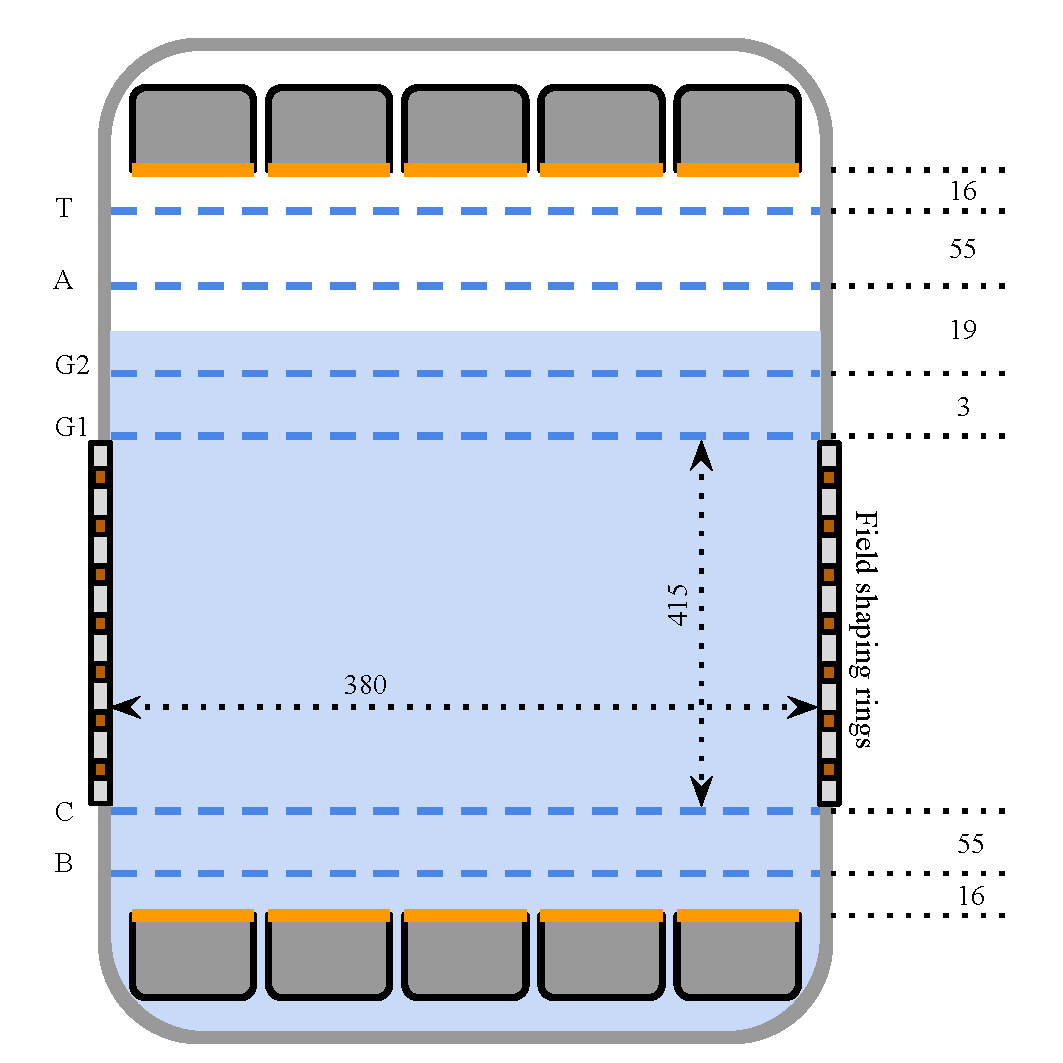
\includegraphics[width=0.49\linewidth]{images/red100grids.pdf}
  \hfill
  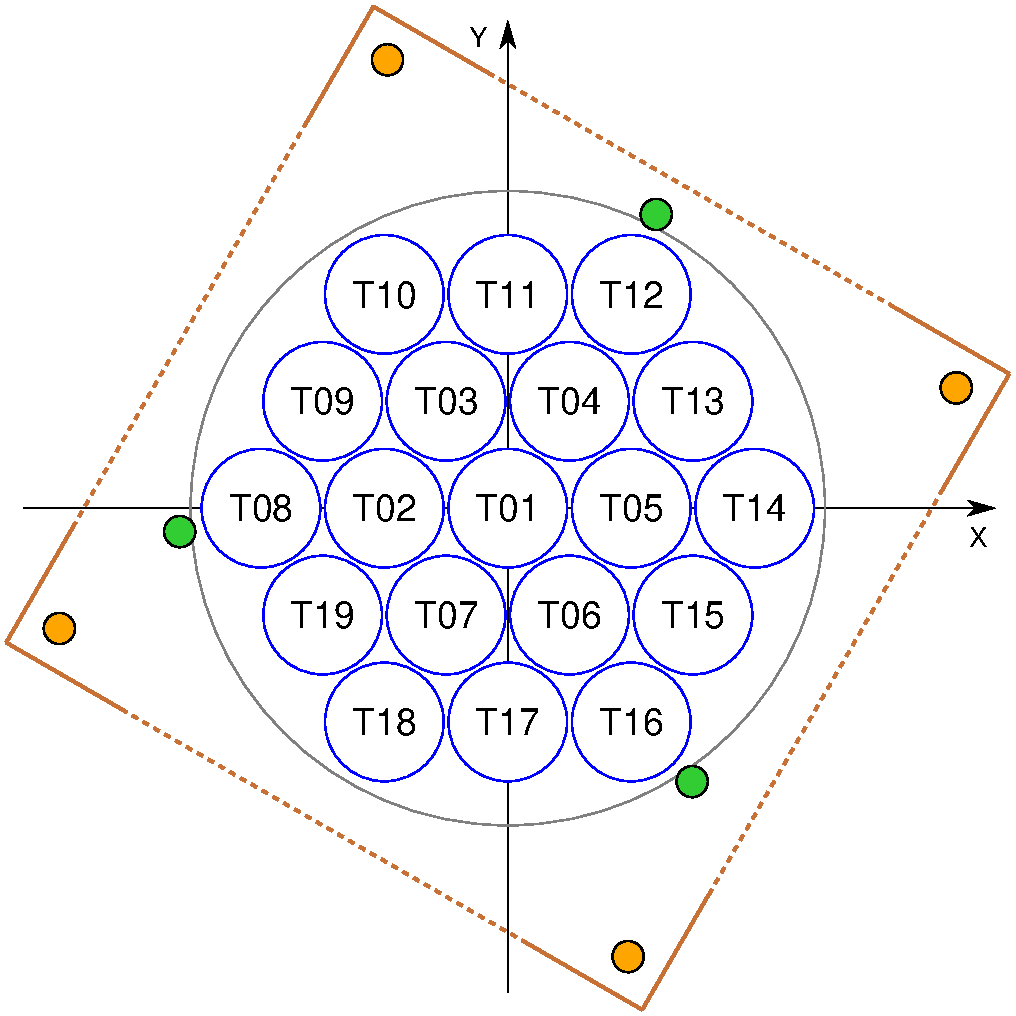
\includegraphics[width=0.46\linewidth]{images/PMT_top_fancy.pdf}
  \caption{\textbf{Left}: Geometry of the RED-100 target volume and electrodes. A---anode; C---cathode; B,T---shielding electrodes; G1---shutter electrode, G2---extraction grid. Dimensions are given in millimeters. \\ \textbf{Right}: Scheme of PMT layout in the top array. Green circles indicate LEDs location. Brown lines indicate the edges of the copper passive shield. The dashed part of these lines indicates that the shielding is drawn out of scale. The length of the inner side of the square is 75 cm. Orange circles indicate source tubes positions.}
  \label{img:red100geometry}  
\end{figure} 

The energy deposited in the interaction of an ionizing particle with a target medium goes mostly to scintillation (S1) and ionization. The S1 signal is caused by the deexcitation of excited states of formed Xe dimers and occurs shortly after the moment of interaction. Part of the ionization electrons recombines and contributes to the S1 signal by forming Xe dimers, whereas the electrons that escape recombination drift towards the surface of the liquid under the applied electric field.
During the drift, they can be captured by electronegative impurities, leading to a characteristic exponential decrease of the signal. At the surface, the electrons are extracted to the gas phase due to the higher electric field generated by the "gate" grid and the anode, or they can remain trapped under the surface \cite{Akimov:2012zz}. Extracted electrons produce a delayed electroluminescence signal (S2) in the gap between the surface and the anode grid~\cite{Aprile:2008bga}. The electrons that were originally trapped or captured by electronegative impurities can later escape and contribute to the specific background in the form of spontaneous emission of single electrons \cite{Akimov_2016_delayed_electrons, PhysRevD.102.092004, Kopec_2021}.

\cevns{} events have very low energy; in this region, S2 appears as a pack of individual single photoelectron (SPE) signals scattered over a noticeable time span and across many channels. 
%
To effectively handle this situation, fast electronics are used, and detailed waveforms with a sampling period of 2 ns are recorded for all PMTs by the data acquisition system (DAQ) for further processing and analysis \cite{Akimov2017}. The recorded time window varies for different types of measurements but typically equals 300 $\mu$s, which is larger than the maximum drift time of 265 $\mu$s. The trigger is either external from the pulse generator or internal from the leading-edge discriminator, tuned to start from S1 and run on a sum of bottom PMTs.

The simulation of the expected signal and data analysis require a precise understanding of the processes in the detector. For this purpose, the following quantities have to be obtained:

\begin{itemize}
    \item single photo-electron (SPE) signal area for each PMT,
    \item single ionization electron (SE) signal parameters (time duration and number of SPEs per SE),
    \item light response functions of PMTs,
    \item electron lifetime,
    \item visible ionization yield (number of ionization electrons passed to the electroluminescence gap),
    \item efficiency of electron extraction from liquid to the gas gap (EEE).
\end{itemize} 

A comprehensive calibration program included several different types of measurements:
%
\begin{enumerate}
    \item \textbf{LED (light-emitting diode)} calibration. Three LEDs were located in the detector as shown in figure~\ref{img:red100geometry}. The LEDs were powered by low-intensity wide pulses from the generator to produce separated SPE signals in all channels. The LED pulses and the trigger were synchronized and were running at 2 Hz. This calibration data was used to measure SPE pulses and calculate SPE parameters for each PMT.

    \item \textbf{SE calibration.} The SE data were collected using an external trigger from the 2 Hz pulse generator. The main objective of this data was to facilitate the observation of accidental SPE signals and spontaneous SE events without any hardware threshold, which is very important for very low-energy signals such as SE. 
    
    \item \textbf{Muon calibration.} Due to minimal shielding from the cosmic background, an intense flux of cosmic ray muons is present at the detector location unlike other experiments with two-phase noble gas detectors. Hence, this flux can be used as a fast and reliable method of the mean electron lifetime measurement. Atmospheric muons are energetic and can pass through the detector, leaving a continuous ionized track along the path. When many individual muon signals are summed up, the resulting signal represents the average dE/dx, which is constant throughout the detector depth. The drift speed doesn't depend on the source of ionization or deposited energy. The signal shape follows exponential decay with drift distance because of finite electron lifetime, which can be obtained as described in~\cite{lifetime}. This method of the lifetime measurement was compared with other methods, and the agreement was demonstrated~\cite{7027252}. The evolution of the lifetime throughout the RED-100 run at KNPP, measured using cosmic muons, can be found in~\cite{The_RED100_Experiment}. 

    \item \textbf{Gamma calibration.} Radioactive sources $^{60}$Co and $^{137}$Cs were placed inside the passive shielding via the guide tubes as illustrated in figure \ref{img:red100geometry}. The sources were aligned with the center of the detector's sensitive volume in a vertical direction. This calibration was performed once per week during the entire RED-100 data-taking period. The main objectives of this calibration included the verification of the stability of the detector parameters and the performance of the energy calibration. Another important goal was to measure the light response functions (LRFs) of the PMTs.

\end{enumerate}



\section{Data processing and analysis}
\label{sec:processing}
\subsection{REDOffline}
\label{sec:RED offline}
The dedicated software package REDOffline was developed by the collaboration for data processing. This lightweight and flexible solution features a modular design that benefits from the use of ROOT libraries \cite{BRUN199781} for various tasks. REDOffline converts raw waveform data into physical information about detected signals through a series of steps.

Initially, the baseline is corrected to remove the remaining DC offset and low (18 kHz) frequency pickup noise. The correction is achieved by constructing a spline approximation of the baseline and subsequently subtracting it. The spline knots are placed every 3.75 $\mu$s, which is wider than the measured S2 width to ensure that individual SE or S2 signals do not violate the procedure.

   A simple over-threshold software trigger is applied for pulse detection. The threshold is individual for each channel and is based on the measured noise level in that channel. The typical threshold value is about 1.8~mV. The pulse time region is set slightly wider than the threshold range to account for pulse samples below the threshold. Additionally, there is a limitation that the pulse duration must be at least 40 ns. For each pulse, multiple parameters are evaluated, including amplitude, area, start time, and duration. The pulse area is calculated as a simple sum of waveform samples within the pulse time region multiplied by the sampling period. The effective threshold for pulse finding is low enough to detect SPEs with an efficiency of about 97\%.
   
The clustering procedure groups pulses related to the same physical signal---significantly large S1 and S2 signals from $\gamma$-events and groups of SPE pulses from SE---in one or many channels. The algorithm varies depending on the type of signal and is described in the corresponding sections below.

\subsection{LED-calibration}
\label{subsec:LED}

This type of data requires only finding SPE pulses and calculating their parameters. 
The SPE pulses were defined as pulses with a signal amplitude of more than 2 mV and a duration (full width at half amplitude) of more than 4~ns. 
This unified amplitude threshold is used since PMT voltages are tuned to keep SPE amplitudes approximately the same for all channels. 
As one can see in the example waveform shown in figure \ref{img:spe_shape_eff} (left), some part of the SPE pulse is outside of the determined pulse time window width, which was mentioned in the previous paragraph. The red line on the plot shows the average shape of SPE signal and it lies below the baseline level in the region after the right defined border of the pulse.
It is a complicated problem to account for this part since the amplitude in this region is very close to the noise level.
The ordinary extension of the integration region leads to the degradation of resolution and pulse separation.
 This feature of the signal introduces an additional source of systematic bias in SPE area calculation. 
In the case of large signals, when individual SPE signals are combined into one big pulse, these trailing pieces are included in the total sum.

An example of the pulse area distribution is shown in figure~\ref{img:spe2022}, left.
As one can see, the SPE peak is well-separated from the pedestal, thereby permitting fitting by two Gaussians (for single and double SPE pulses). 
The second peak can be caused by double photo-electron emission~\cite{Faham_2015}, or simple coincidences.
The mean SPE value for each channel, derived from the fit, was used to quantify the areas of all other signals in PE units using the efficiency coefficient described below. 

To estimate the area losses, the toy Monte-Carlo simulation was performed. We measured the average SPE signal shape using a high sampling rate oscilloscope. 
Then, a known number of SPE pulses, distributed uniformly in 2~$\mu$s (a characteristic SE signal), was added to the real waveforms without detected pulses. 
The number of the SPE pulses was varied from 1 to $10^6$. 
The constructed waveforms were then processed by REDOffline as usual.
As shown in figure~\ref{img:spe_shape_eff}, right, there is a significant decrease in area calculation efficiency for SE-like signals represented by sparce SPE pulses. 
The asymptotic value of this efficiency for SPE is 81$\pm$1\%, which coincides with direct integration of SPE signal shape using average pulse time window width for SPE pulses. 

\begin{figure}[htbp]
 \centering
 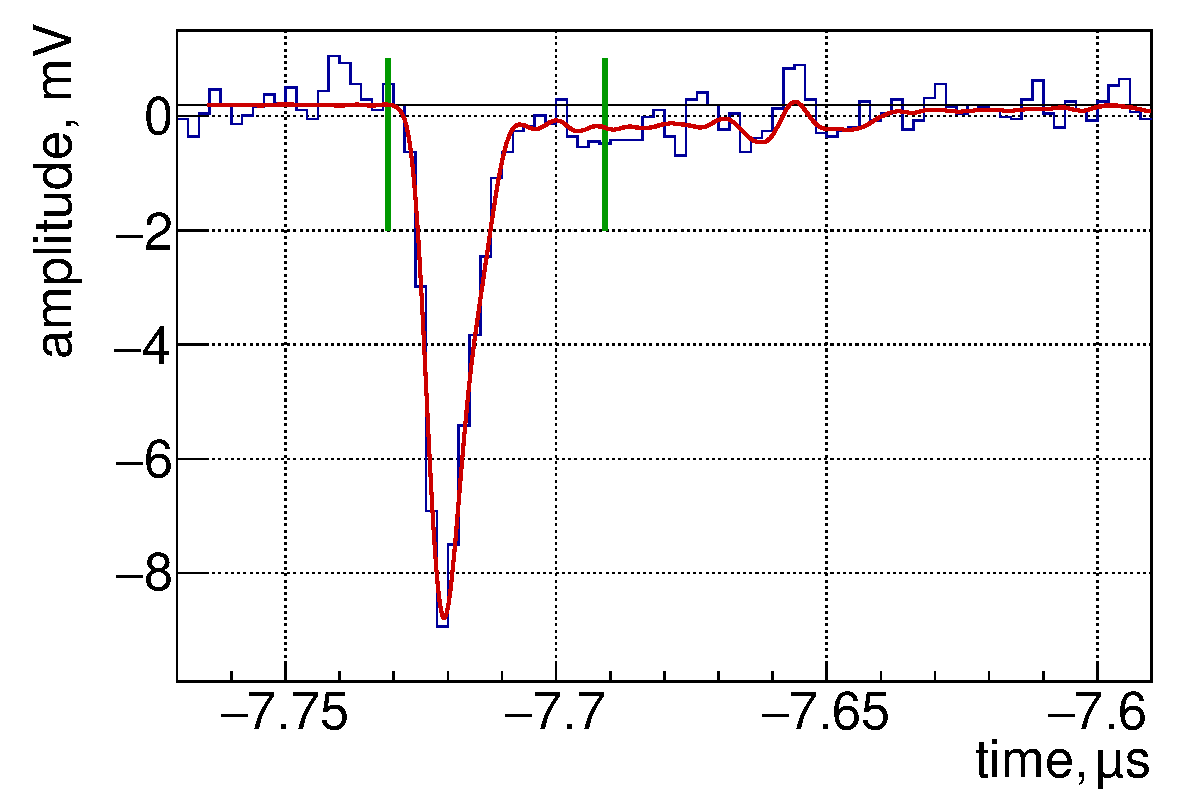
\includegraphics[width=0.49\linewidth]{images/spe-519-63-t01-fix.pdf}
 \hfill
 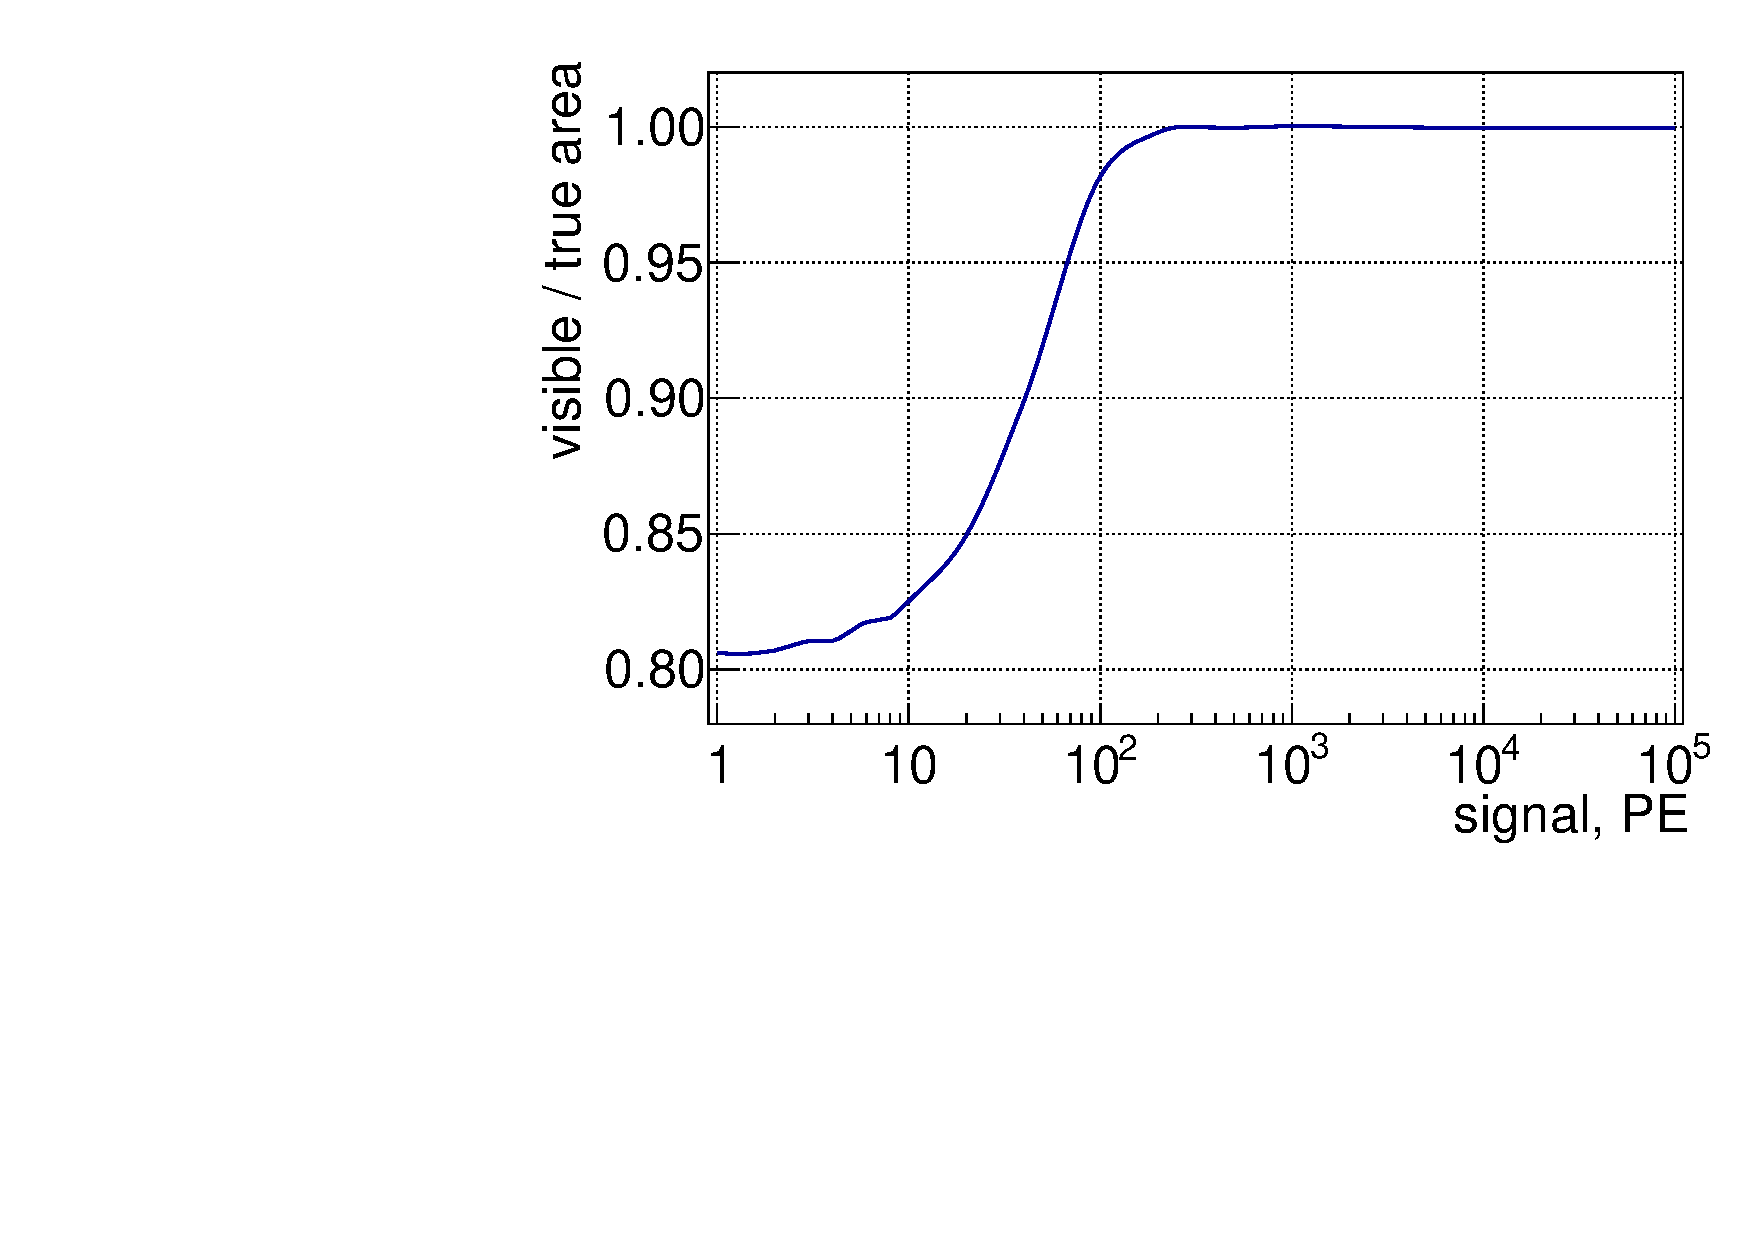
\includegraphics[width=0.49\linewidth]{images/spe_area_eff.pdf}
	\caption{\textbf{Left}: Example of the waveform with SPE signal on it. Green lines indicate borders of the identified pulse. The red line indicates the measured averaged shape of the SPE pulse. \textbf{Right}: The efficiency of the pulse area evaluation depending on the number of PE generated per event.}
  \label{img:spe_shape_eff}  
\end{figure}

During the scientific data collection period, slow variations of the mean SPE area were observed. 
It was accounted for by fitting the time dependence of the mean SPE area with a linear function, as shown in figure~\ref{img:spe2022}, right. 
In further analysis, the value of this function for a particular run was used as the SPE size.

\begin{figure}[htbp]
  \begin{minipage}[ht]{0.49\linewidth}    \center{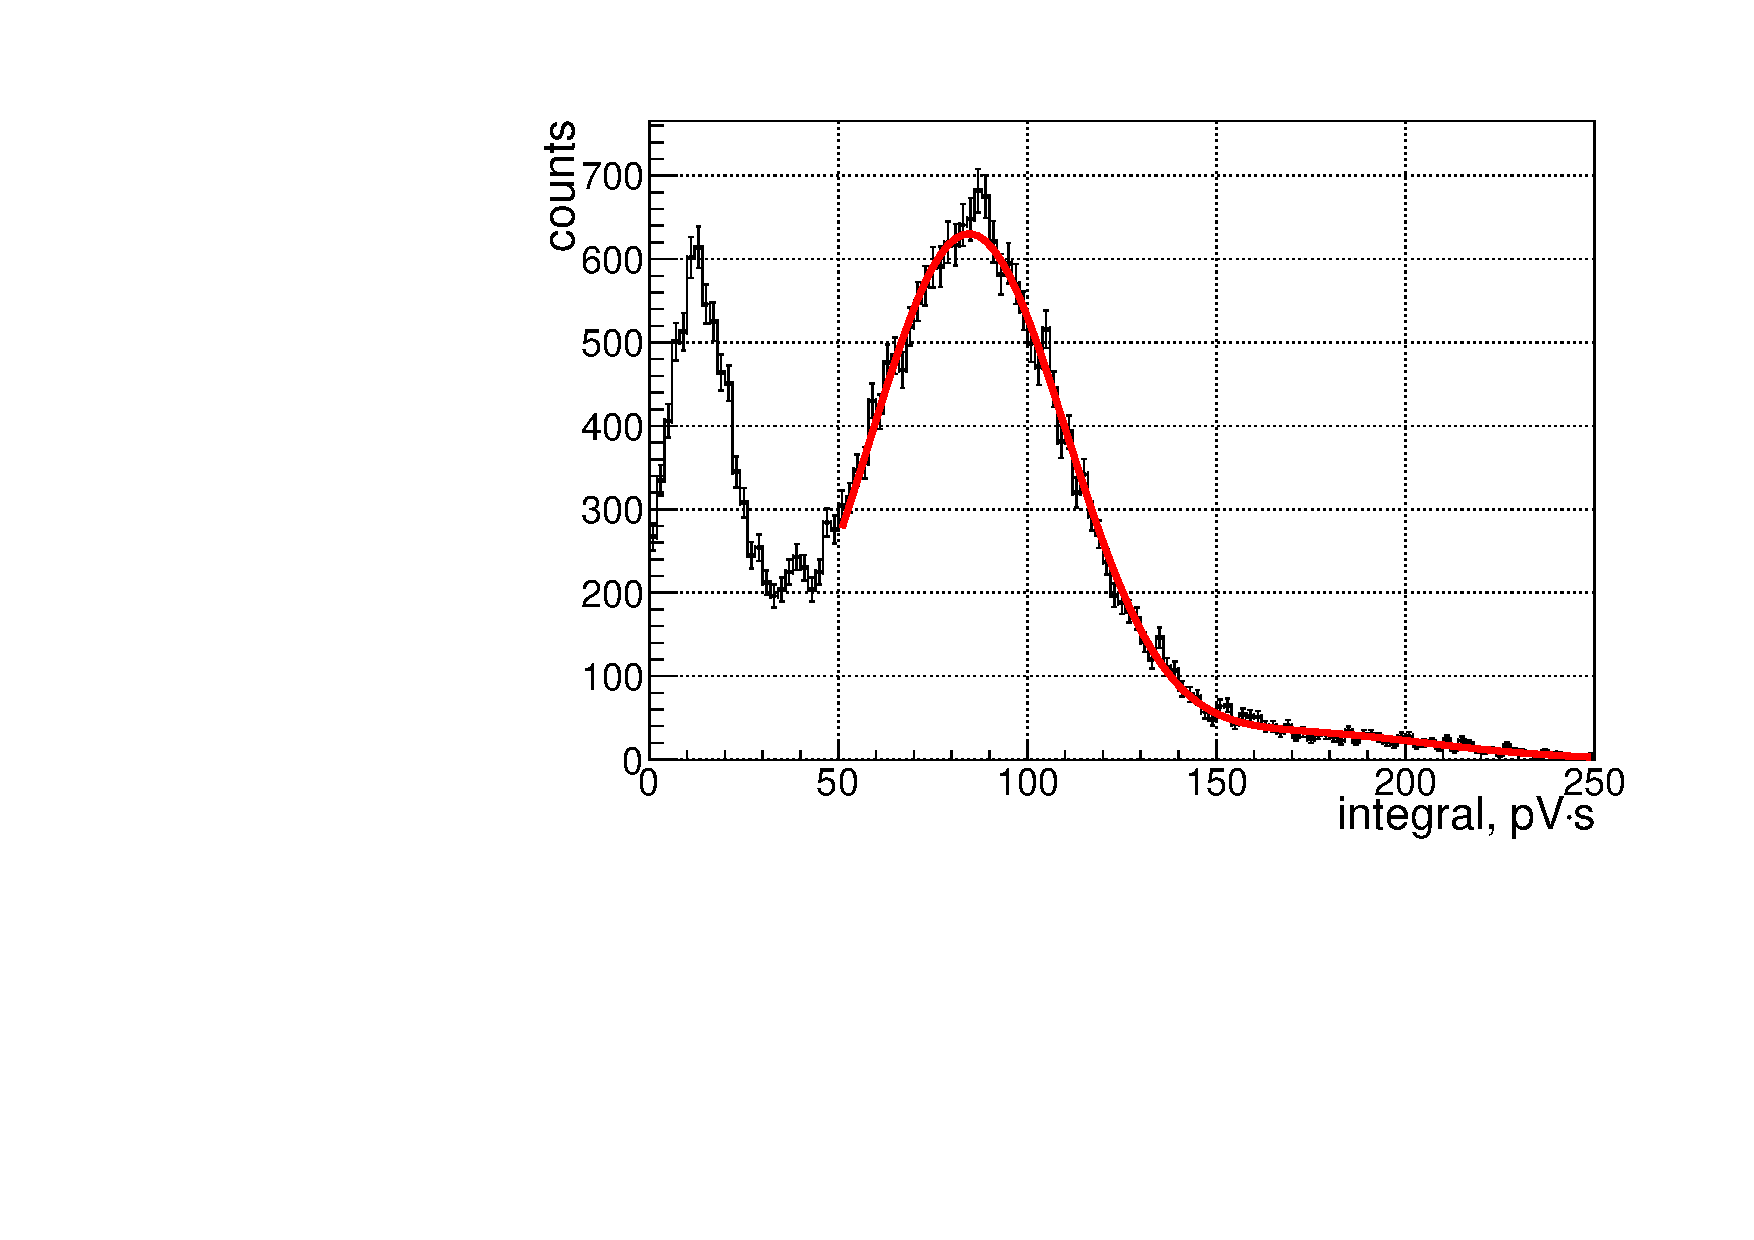
\includegraphics[width=1.0\linewidth]{images/top_09_LED.pdf} \\}
  \end{minipage}
  \hfill
  \begin{minipage}[ht]{0.49\linewidth}  \center{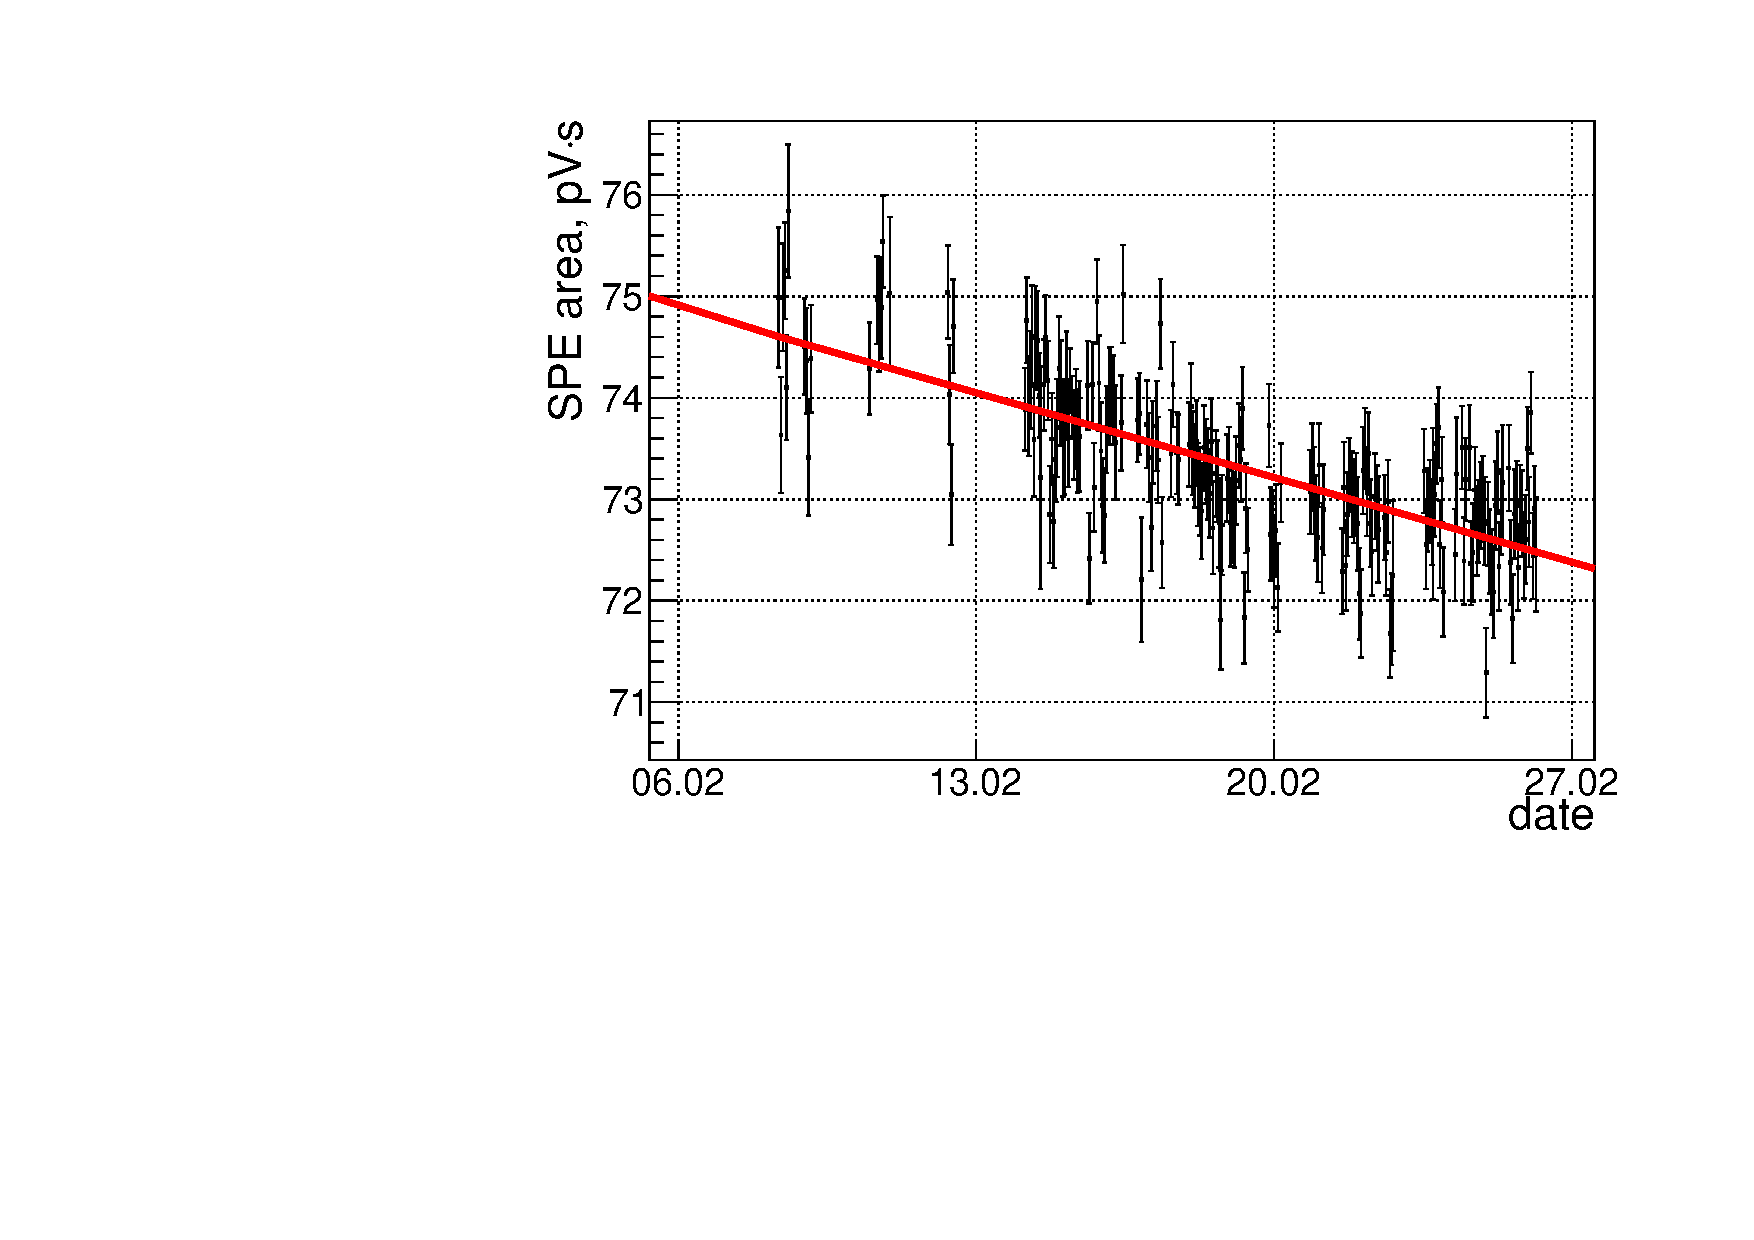
\includegraphics[width=1.0\linewidth]{images/T09_spe_vs_time.pdf} \\}
  \end{minipage}
    \caption{\textbf{Left}: Example of the SPE spectrum for PMT T09 (top array) and the linear fit (red line). \textbf{Right}: Dependence of the mean SPE integral on time for PMT T09 (top array) and the result of the fitting (red line).}
\label{img:spe2022}
\end{figure}

\subsection{SE-calibration}
\label{subsec:SE}

Spontaneous emission of SE taking place in LXe two-phase detectors~\cite{Akimov:2012zz,Akimov_2016_delayed_electrons, PhysRevD.102.092004, Kopec_2021} can be used for the light yield calibration.
The signal from one SE represents the minimal size of electroluminescence and is composed of several SPE pulses uniformly distributed over the entire length of the electroluminescence. 
Consequently, a clustering procedure is required. The SE signal clusters were identified on the waveforms as groups of SPE pulses using the algorithm detailed below:

\begin{itemize}
    \item 
    The pulses with an area larger than the threshold area were selected. 
    The threshold was calculated as two standard deviations down from the mean value of the first Gaussian on the SPE area spectrum. The use of the threshold connected to SPE size instead of the pedestal helps unify the efficiency of the selection relative to SPE in different channels with varying noise levels.
    \item 
    The clusters were formed as groups of pulses from the top PMT array if the time distance between the start times of two consecutive pulses did not exceed 500 ns.
    The duration of a cluster was calculated as the time distance between the onset of its first pulse and the end of the last one.
    \item The clusters having fewer than five pulses were rejected.
\end{itemize}

The duration distribution of the SE candidate clusters is shown in figure~\ref{img:sespectrum}, left.
The peak with a center at $\sim$750~ns corresponds to electron emission at the periphery of the liquid surface.
We discard these edge events since they are outside of the drift region from the active volume. 
For further analysis, the clusters with a duration between 1.3 and 2.2~$\mu$s were selected.
This requirement corresponds to the duration of electroluminescence measured from the S2 data. The SE area distribution in units of PEs is shown in figure~\ref{img:sespectrum}, right.

\begin{figure}[htbp]
  \begin{minipage}[ht]{0.49\linewidth}    \center{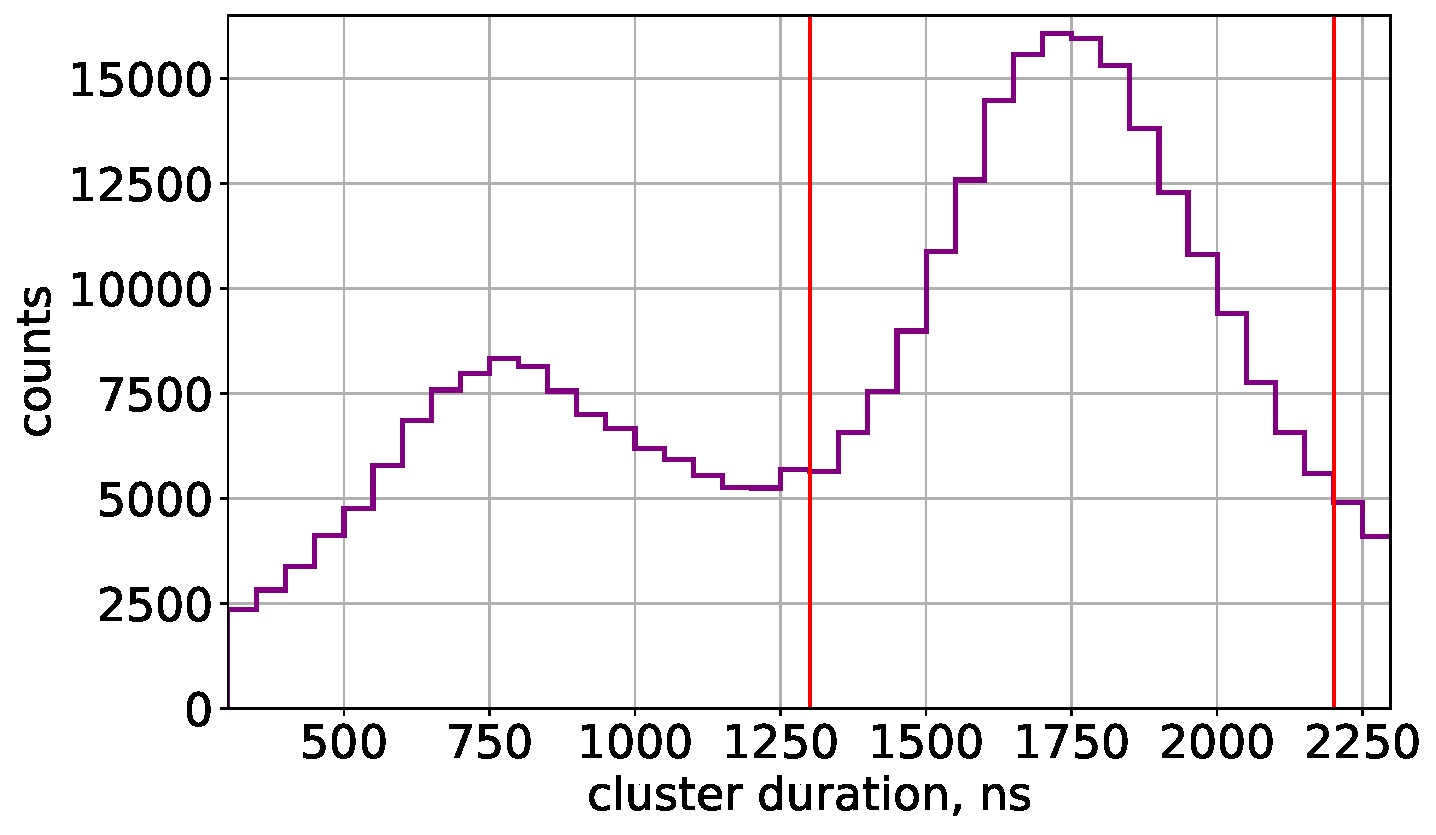
\includegraphics[width=1.0\linewidth]{images/seduration.pdf} \\}
  \end{minipage}
  \hfill
  \begin{minipage}[ht]{0.49\linewidth}  \center{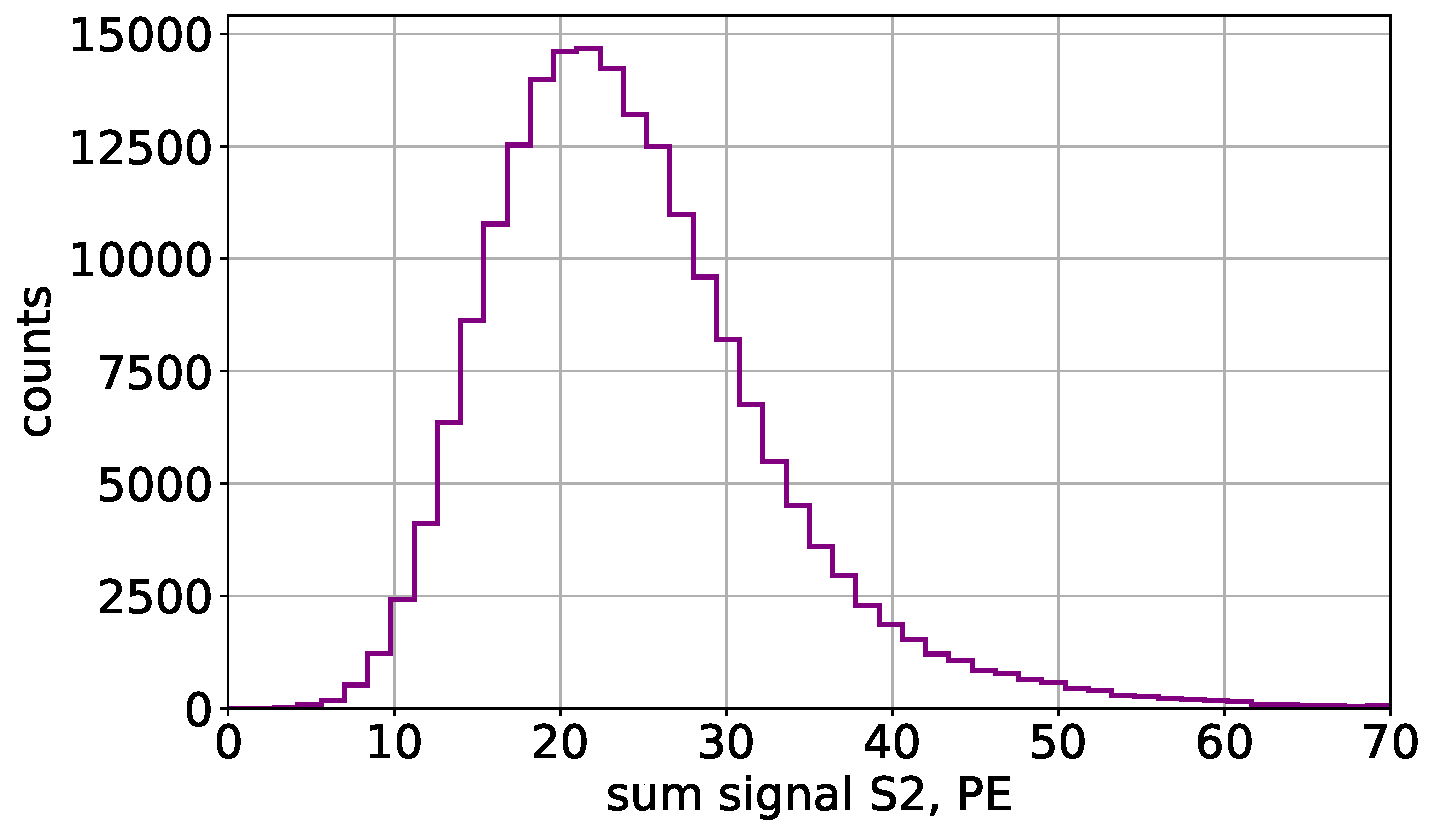
\includegraphics[width=1.0\linewidth]{images/SE_spectrum.pdf} \\}
  \end{minipage}
	\caption{\textbf{Left}: SE duration distribution. The red lines indicate the applied cut.  \textbf{Right}: The SE area distribution in terms of PEs with applied only duration cut.}
	\label{img:sespectrum}
\end{figure}

\subsection{Calibration by gamma-sources}
\label{subsec:gamma}
Gamma calibration analysis requires the selection of pulse groups (clusters) corresponding to S1 and S2 signals on the waveforms. 
The signals from the full absorption peak for the gamma sources we used are large enough to obtain continuous S1 and S2 pulses above the threshold distributed over many channels. 
In this case, a so-called effective summed waveform can be used for data processing. The following algorithm was used to identify S1 and S2 clusters:

\begin{enumerate}
    \item
    The initial pulses were converted to rectangular (with constant amplitude) ones with the same duration.
    The amplitude of these rectangular pulses was calculated by dividing the primary pulse area by its duration. 
    \item The obtained rectangular pulses over all channels were combined into the effective summed waveform.
    \item 
    S1 or S2 on the constructed waveforms were identified using their amplitude and width according to the following criteria: a duration between 70 and 170 ns and an amplitude between 0.2 and 0.9 V for S1,
    a duration of more than 1700 ns and an unrestricted amplitude for S2. 
\end{enumerate}

Afterwards, the so-called full events were constructed using the identified S1 and S2 clusters. 

A two-phase detector technique enables 3-D reconstruction.
The event depth (corresponding to the Z coordinate) can be reconstructed using the time interval between S1 and S2, whereas the XY (horizontal plane coordinates) and energy reconstruction requires a more complex procedure.
The S1 signal depends on the interaction depth because the events closer to the detector's bottom give a greater light response.
This is because the bottom PMT array is more efficient in detecting the S1 signal than the top one due to the total reflection from the surface of a liquid. This depth dependence was mitigated by applying a cubic polynomial correction to the S1 signal. The correction function was measured using $^{137}$Cs data. As mentioned earlier, the S2 signal is depth-dependent due to ionization electron losses. 
The S2 area in each channel was corrected using the electron lifetime obtained from the muon data by the exponential function of depth:
\begin{equation}
A_{{i }}=A_{i \text{ raw}} \cdot e^{{t_{\text {drift}}}/{\tau}},
\end{equation}
where $A_{i \text{ raw}} $ represents the S2 area in $i$-th channel before the correction, $A_{{i }}$---after the correction, $\tau$---the measured electron lifetime, $t_{\text {drift}}$---the time difference between S1 and S2 onsets. 
The events with only one scintillation and only one electroluminescence were selected for analysis. Then, depth and duration cuts were applied. Examples of event distributions on the depth and the duration, along with the corresponding cuts, are shown in figure~\ref{img:depthdur}.

\begin{figure}[htbp]
  \begin{minipage}[ht]{0.49\linewidth}    \center{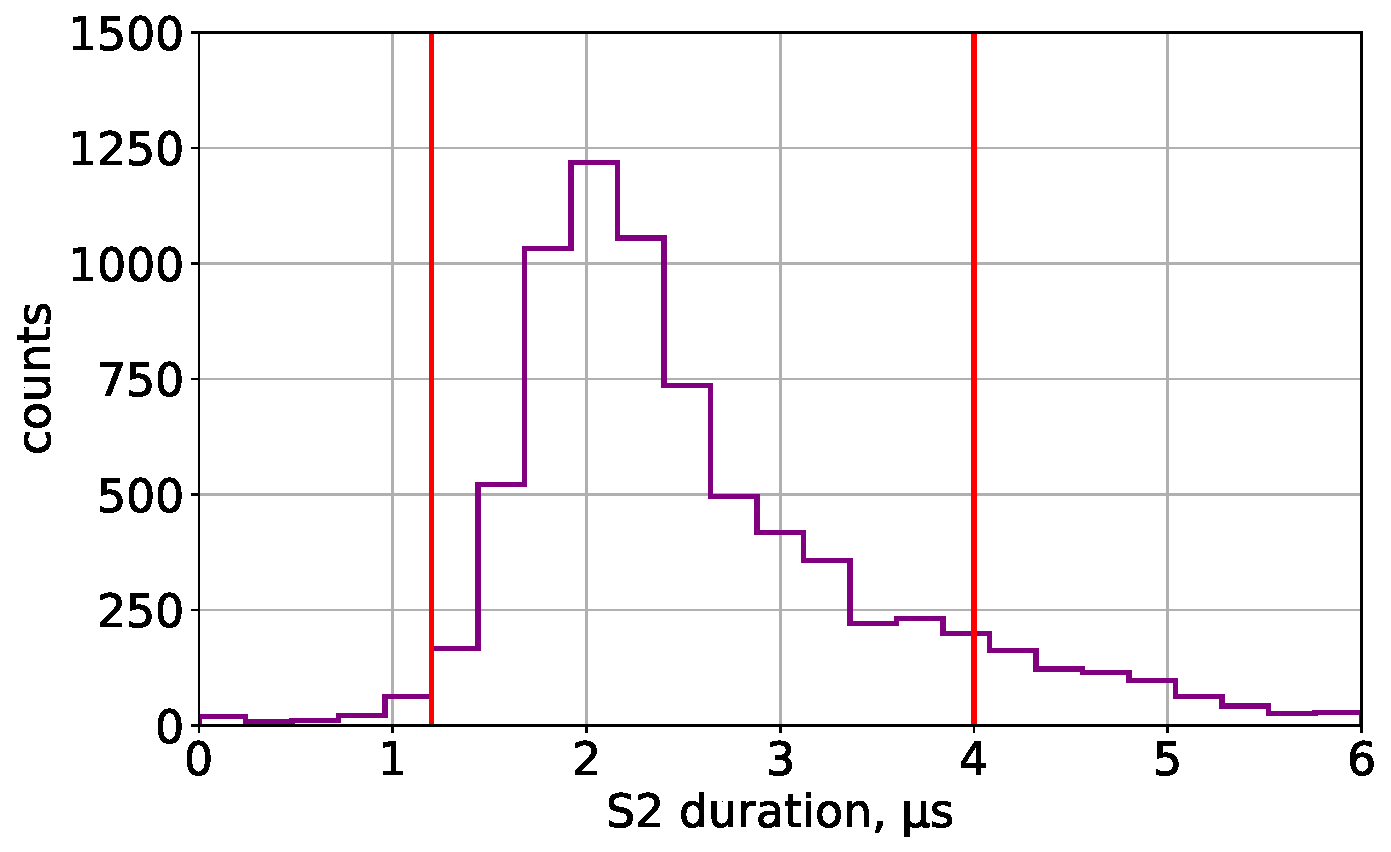
\includegraphics[width=1.0\linewidth]{images/dur_distr_run_877.pdf} \\}
  \end{minipage}
  \hfill
  \begin{minipage}[ht]{0.49\linewidth}  \center{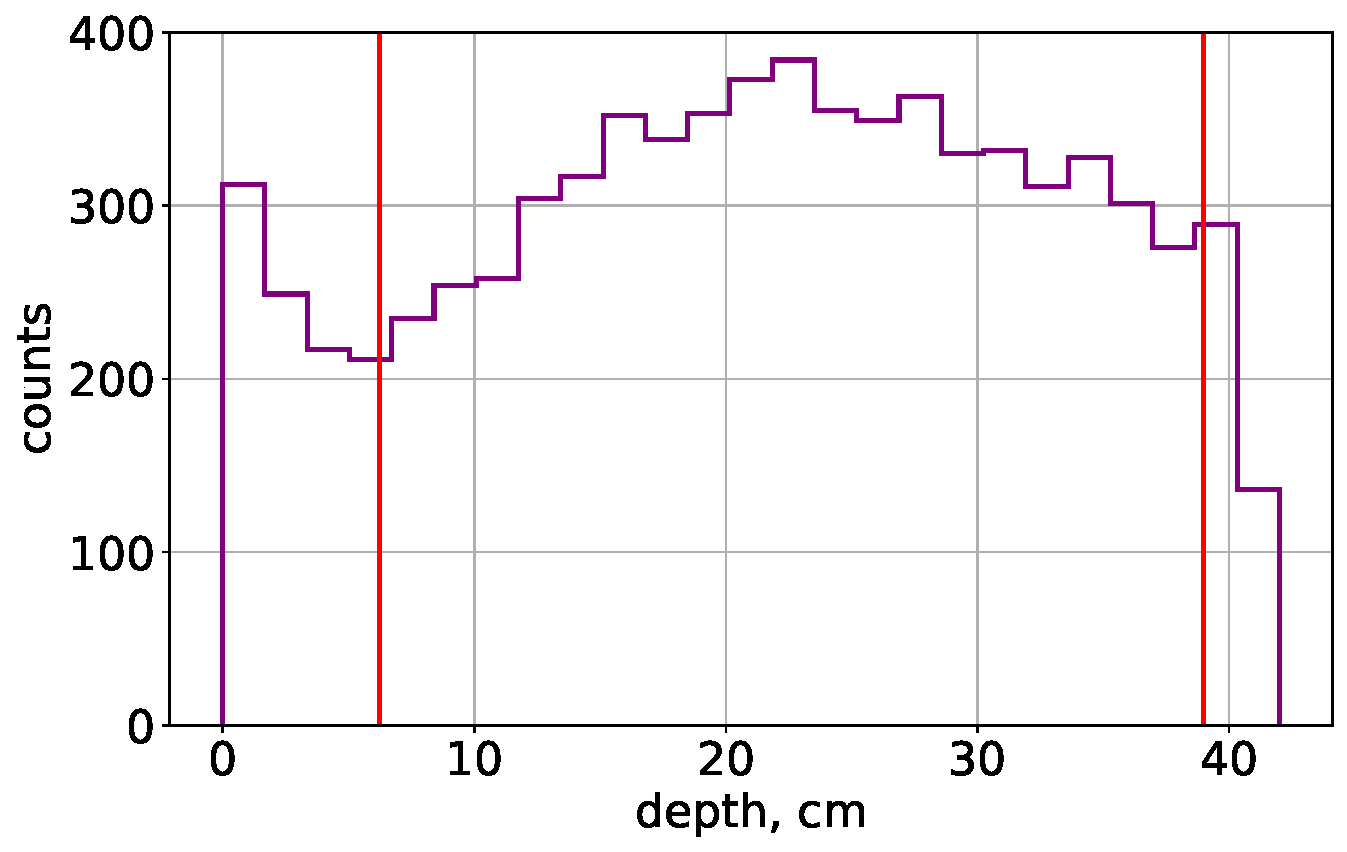
\includegraphics[width=1.0\linewidth]{images/depth_distr_run_877.pdf} \\}
  \end{minipage}
	\caption{\textbf{Left}: The example of S2 duration distribution for the run with gamma source $^{60}$Co. \textbf{Right}: The example of depth distribution for the run with gamma source $^{60}$Co.}
	\label{img:depthdur}
\end{figure}

\subsubsection{Light response functions (LRFs) evaluation}
\label{subsubsec:lrfrec2}
The detector response depends on the event's XY position due to the top PMT array's light collection efficiency.
Events from the region of interest (<10 ionization electrons) of the RED-100 detector have very low energy and do not produce significant S1 signals.
Thus, the correction and reconstruction procedure was performed only for S2 signals.

The center-of-gravity method, also known as the centroid, is the simplest and fastest method for position and energy reconstruction. In this method, the event coordinates are determined as follows:
\begin{equation}
X_{\text {event }}=\frac{\sum_i A_i X_i}{\sum_i A_i}, \quad Y_{\text {event }}=\frac{\sum_i A_i Y_i}{\sum_i A_i},
\end{equation}
where ($X_i$, $Y_i$) represent the coordinates of the $i$-th PMT's axis, and $A_i$ is the measured area of the S2 signal from this PMT.
The energy is reconstructed by summing up the signals from all PMTs from the top array.
This method is effective because PMTs that register the largest signals are typically positioned close to the light emission point on the XY plane.
The centroid method is very fast and relies only on the amount of light collected by each PMT.
Unfortunately, this method has disadvantages; the position and energy reconstruction are distorted near the edges of the detector due to the dependence of the total signal on the radius.
The need for more accurate reconstruction motivates the use of more complex reconstruction techniques.

The reconstruction method we chose is based on the use of LRFs~\cite{Solovov2012} for each PMT.
LRF is a dependence of the PMT signal on the relative light source position to the center of the PMT's photocathode.
In simple cases, only one dimension (radius) is considered, which corresponds to the projection of the distance between the PMT and the light source on the XY plane. 
More complex cases utilize two (XY or RZ) or three (XYZ) dimensions. 
In our analysis, we employed 1-dimensional LRFs (figure~\ref{img:xy_and_lrf}, left).
All methods involving LRFs operate under the assumption that the LRF shape is independent of the light amount in the linear operation mode of the PMT. 
There are several ways to determine the LRF shape, such as Monte-Carlo simulation, analytical calculations, or analysis of experimental data. Sometimes, a combination of these approaches is used.

For the LRF reconstruction procedure, we used the Mercury~\cite{Solovov2012} iterative algorithm on $^{60}$Co experimental data. 
Events only from the energy region of two close photopeaks from 1173 and 1333~keV were used. 
These events were chosen because they have well-defined energy. 
The environment for the LRF evaluation procedure is implemented in ANTS2~\cite{Morozov_2016}, a software package designed for the position, energy reconstruction, and optical modeling of detectors. 
It also includes the implementation of the LRF fitting and various reconstruction methods, one of which was used in our analysis. The specific implementation of it is described below.

\begin{figure}[htbp]
  \begin{minipage}[ht]{0.36\linewidth}    \center{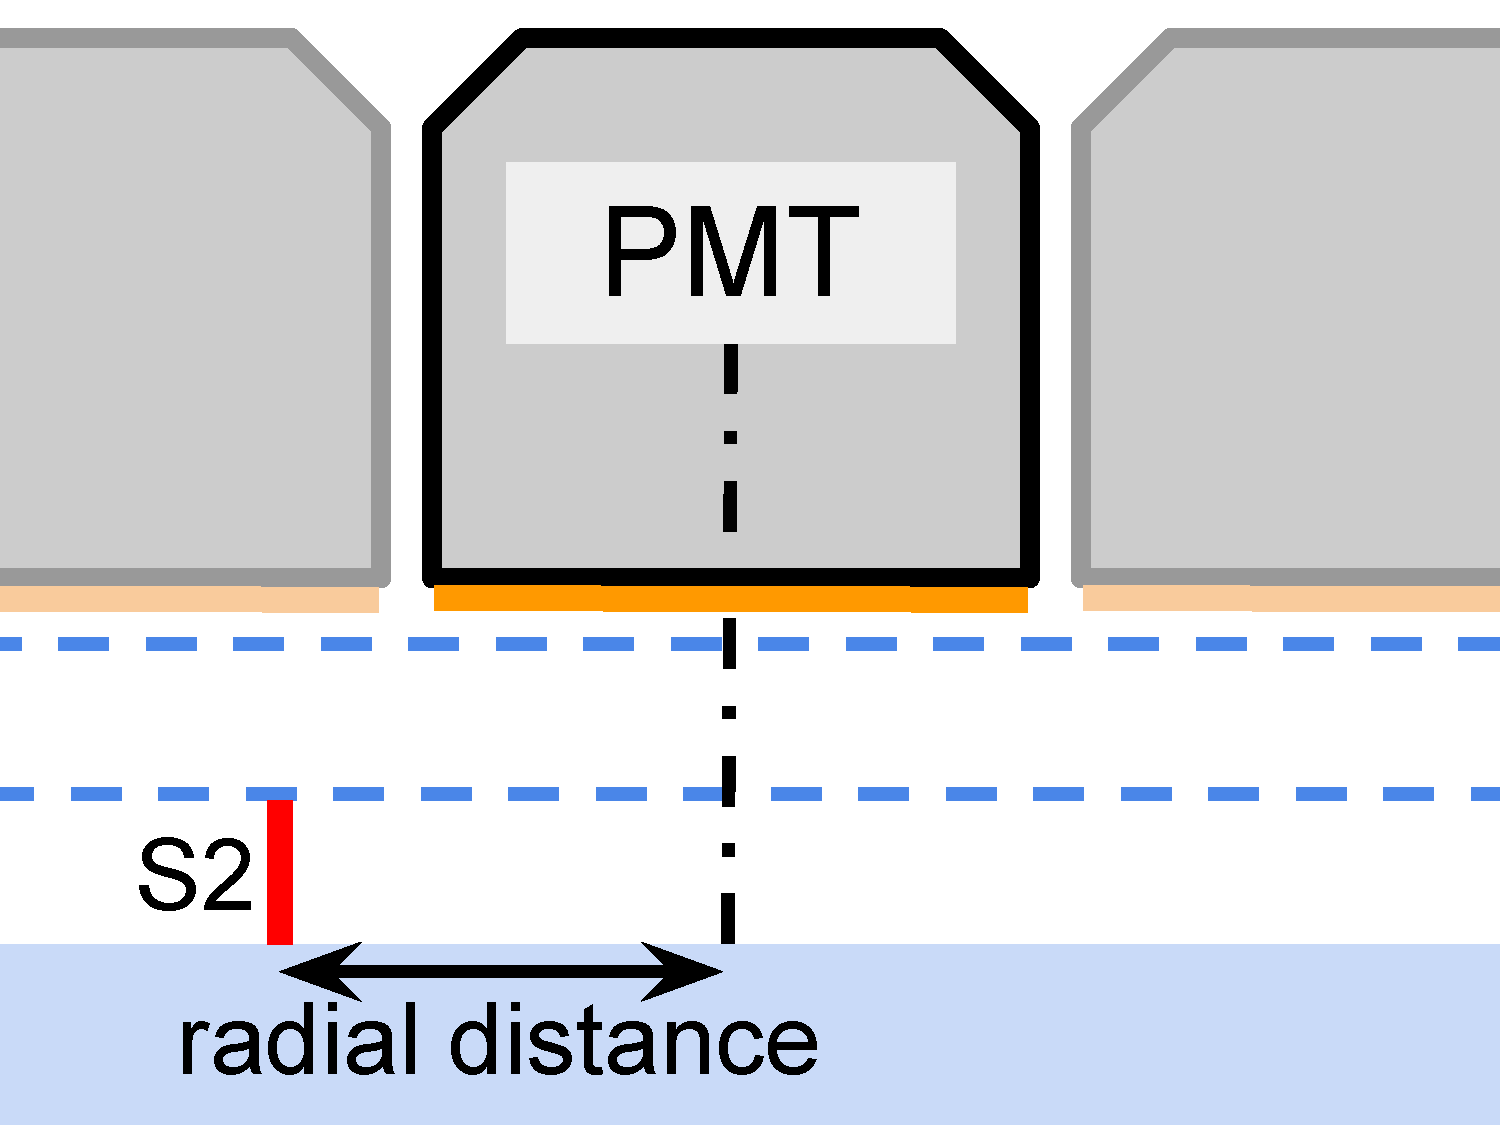
\includegraphics[width=1.0\linewidth]{images/LRF_pmt_old.pdf} \\ }
  \end{minipage}
  \hfill
  \begin{minipage}[ht]{0.62\linewidth}  \center{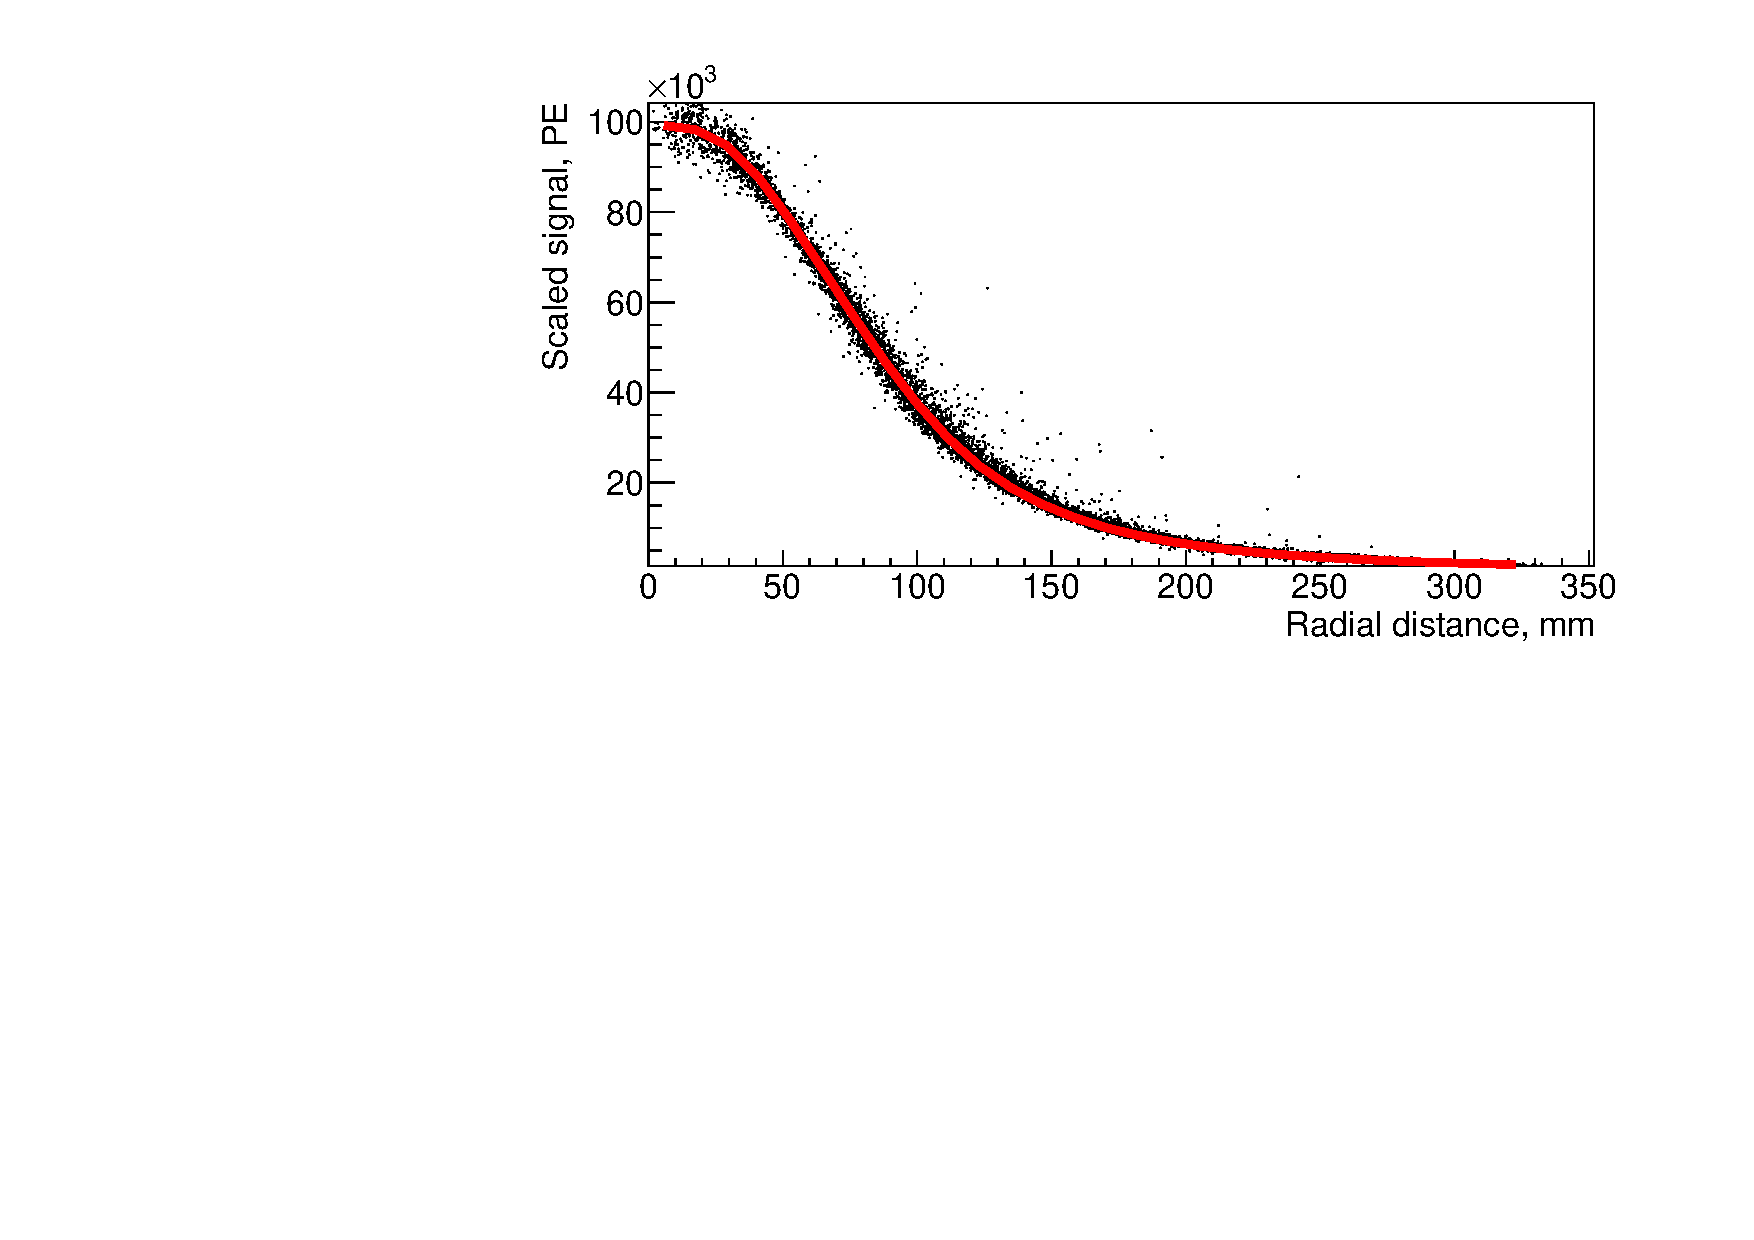
\includegraphics[width=1.0\linewidth]{images/lrf15_pic.pdf} \\ }
  \end{minipage}
	\caption{\textbf{Left}: The scheme of the radial distance measurement. \textbf{Right}: The example of the reconstructed LRF (red line) and signal distribution for PMT T16. The signal is multiplied by the energy calculated using the formula~\ref{Energy_formula}.}
	\label{img:xy_and_lrf}
\end{figure}
%
\begin{figure}[htbp]
    \center{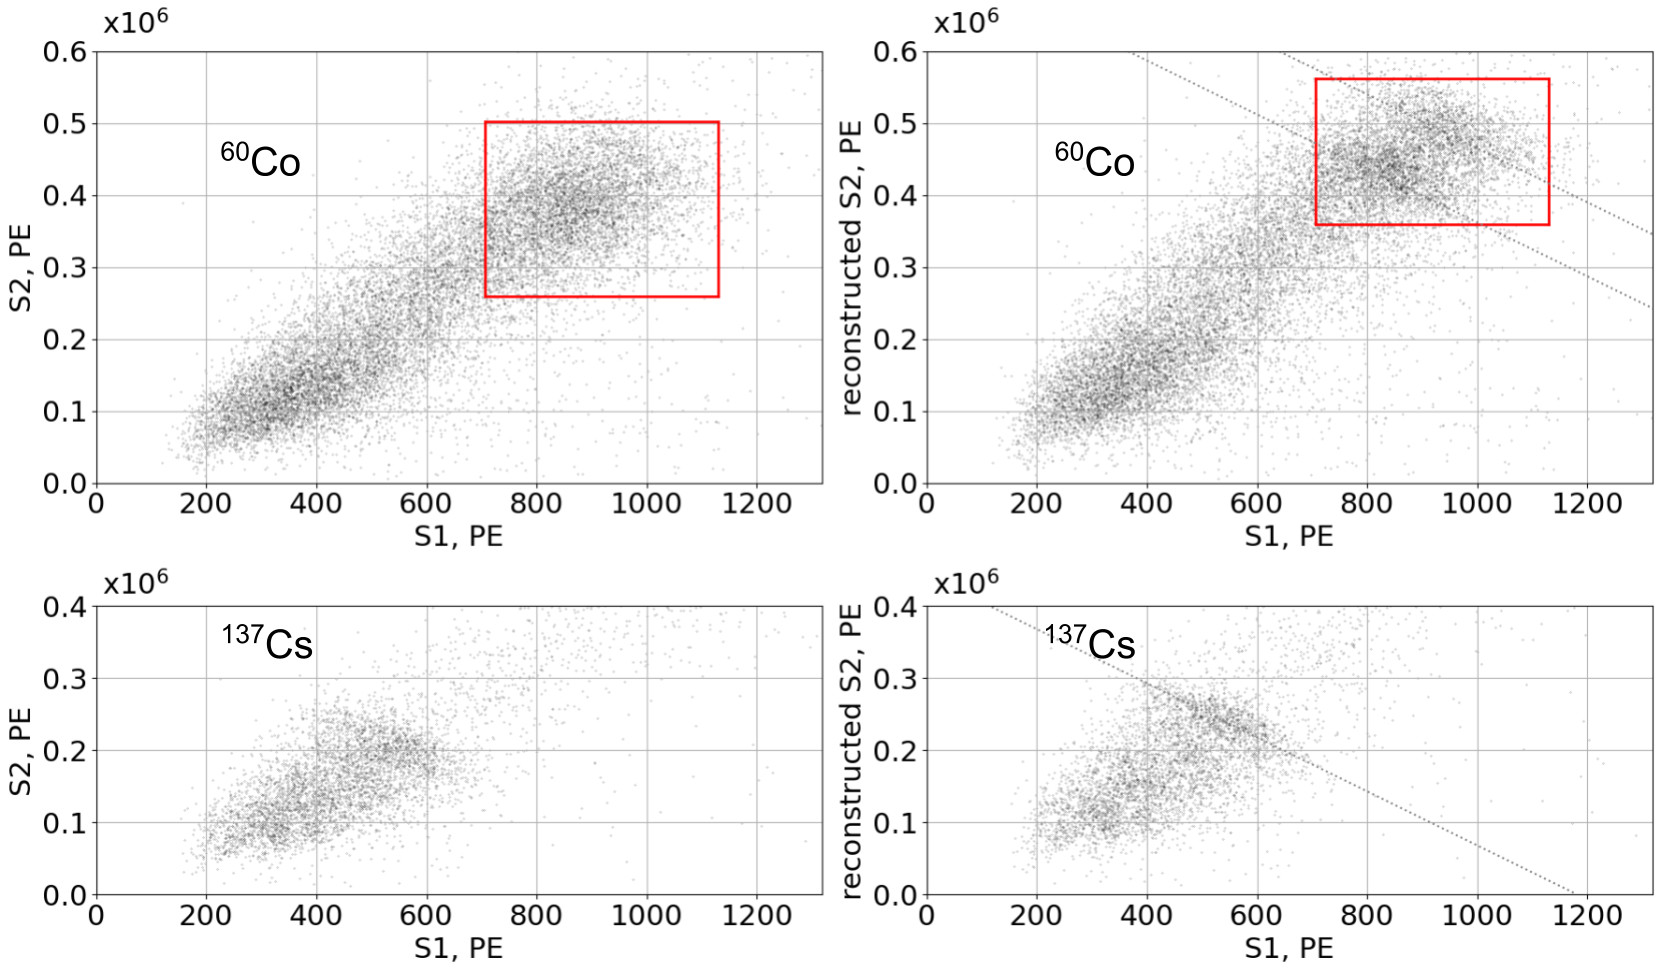
\includegraphics[width=1.\linewidth]{images/Co_Cs_2d_sp-3.png} \\}
	\caption{\textbf{Left}: S2 vs S1 scatter plot before reconstruction.
 \textbf{Right}: S2 vs S1 scatter plot after reconstruction. \\The $\chi^2$ and the R cuts are applied to the events on both distributions. The red lines show selection of the events taken into LRF reconstruction. The grey dotted lines indicate the selected $^{60}$Co and $^{137}$Cs peaks.}
  \label{img:2dspectra}  
\end{figure}
%
On each iteration, the distributions of the signal on distance from the PMT's axis were fitted by B-splines to obtain LRFs. 
The coordinates for the first iteration were calculated using the centroid method and then multiplied by an empirical coefficient of 1.8 to scale the distribution to the detector size. 
For subsequent iterations, the maximum likelihood estimation method with contracting grids~\cite{grids} was applied for XY reconstruction of all events. The likelihood function was computed as follows:
%
\begin{equation}
L_{\text {event }}=-\sum\limits_{i=1}^{19} \Big( A_i \ln(LRF_i(x,y) E) - LRF_i(x,y) E \Big),
\end{equation}
where $A_i$ is the measured S2 signal area from the $i$-th PMT of the top array, $LRF_i(x,y)$ is the LRFs value from $i$-th PMT corresponding to the reconstructed coordinates $x,y$, and $E$ represents the reconstructed energy, which was calculated as:
\begin{equation}
\label{Energy_formula}
E_{\text {event }}={\sum\limits_{i=1}^{19} A_i}\Big{/}{\sum\limits_{i=1}^{19} LRF_i(x,y)},
\end{equation}
  
The S2 versus S1 scatter plots before and after reconstruction with corresponding event selection are shown in figure~\ref{img:2dspectra}.
Reconstructed S2 energy in PEs was calculated as the energy from~\ref{Energy_formula} multiplied by the coefficient between reconstructed and measured S2. 
This coefficient was calculated using the events from the central area of the detector. 
The distributions presented in figure~\ref{img:2dspectra} were obtained after applying the sum $\chi^2$ and the radius cuts, which are described below. 
An example of the measured LRF is shown in figure \ref{img:xy_and_lrf} (right). 

\subsubsection{Event reconstruction}
\label{subsubsec:rec_res}
LRFs make it possible to reconstruct the position and energy for any type of data. 
Reconstruction was performed using the contracting grids method with likelihood maximization for $^{137}$Cs, $^{60}$Co and SE data. Furthermore, this method can be applied to the reconstruction of both experimental and simulated \cevns{} events.

\begin{figure}[htbp]
  \begin{minipage}[ht]{0.49\linewidth}    \center{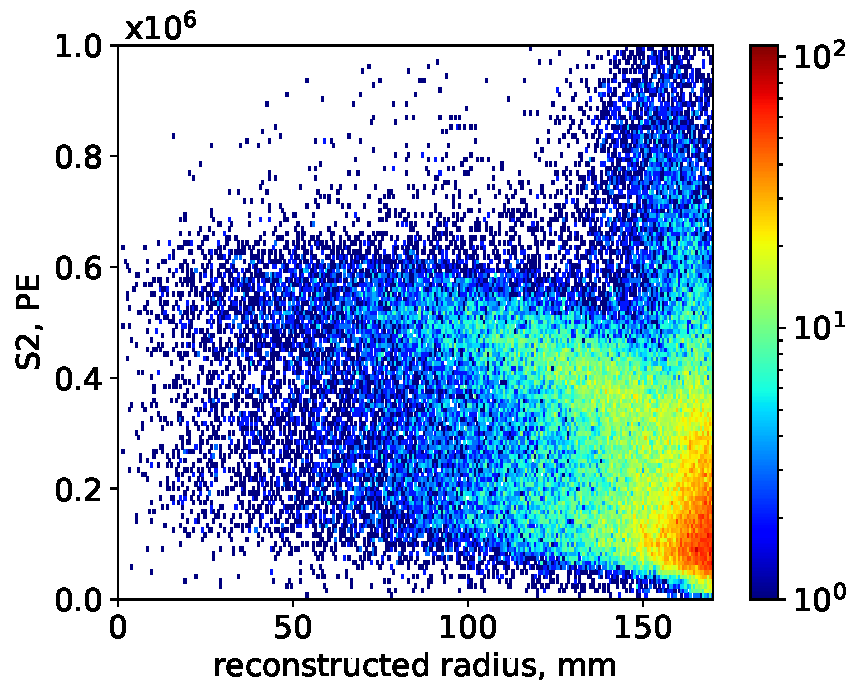
\includegraphics[width=1.0\linewidth]{images/ssum_vs_r.pdf} \\}
  \end{minipage}
  \hfill
  \begin{minipage}[ht]{0.49\linewidth}  \center{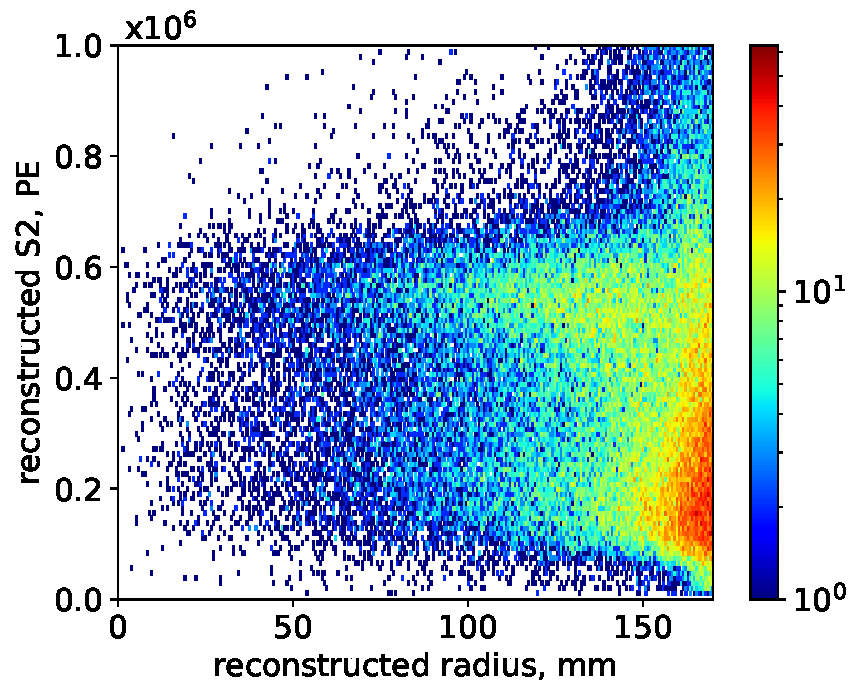
\includegraphics[width=1.0\linewidth]{images/s2_vs_r.pdf} \\}
  \end{minipage}
	\caption{\textbf{Left}: Dependence of the top array sum signal on the reconstructed radius for $^{60}$Co calibration events.
 \textbf{Right}: Dependence of the reconstructed S2 energy on the reconstructed radius for $^{60}$Co calibration events.}
	\label{img:energy_vs_r}
\end{figure}

\begin{figure}[htbp]
  \begin{minipage}[ht]{0.45\linewidth}    \center{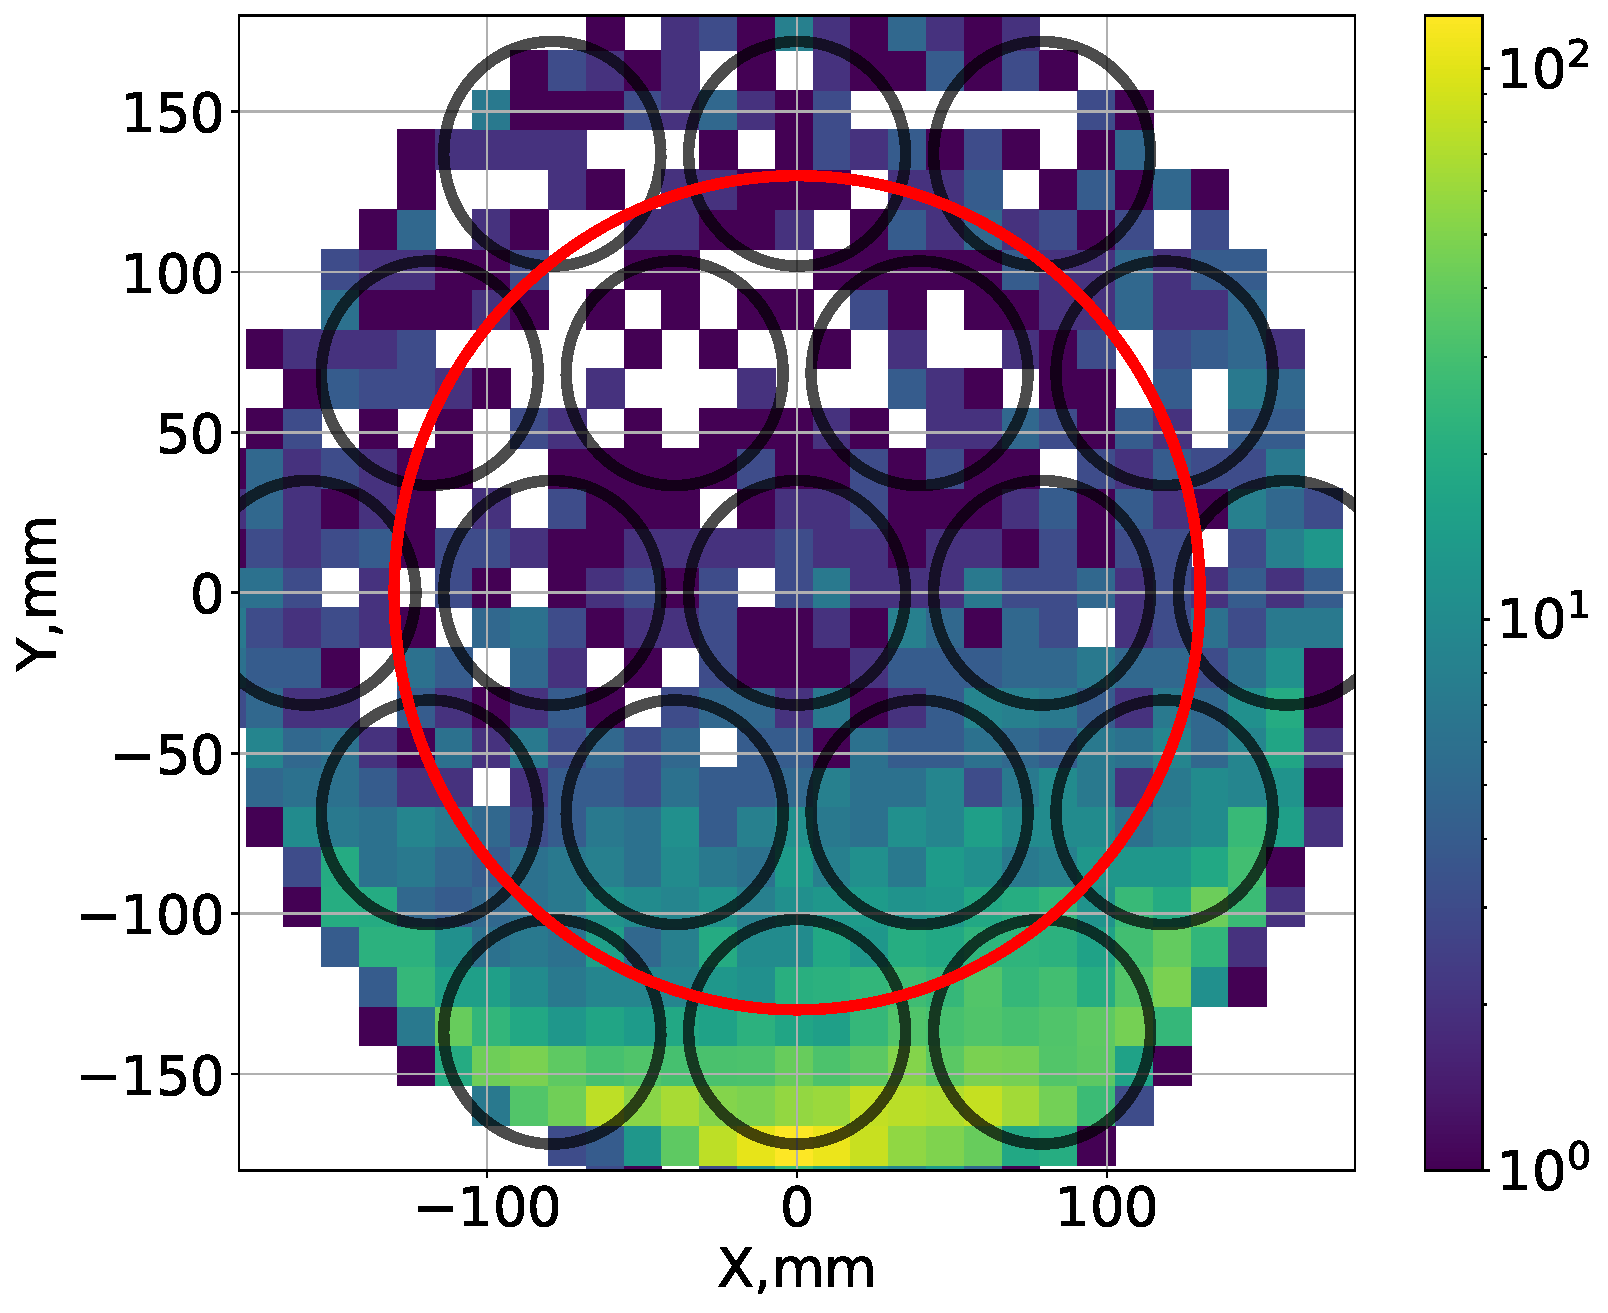
\includegraphics[width=1.0\linewidth]{images/XYhist.pdf} \\}
  \end{minipage}
  \hfill
  \begin{minipage}[ht]{0.53\linewidth}  \center{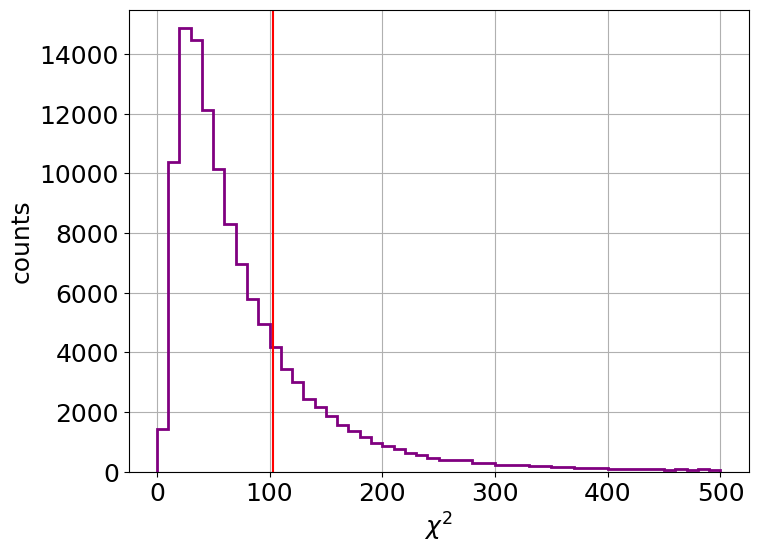
\includegraphics[width=1.0\linewidth]{images/chi2_all.png} \\}
  \end{minipage}
	\caption{\textbf{Left}: The example of reconstructed XY distribution for calibration source located at one of the points shown in figure~\ref{img:red100geometry}. The red line illustrates the selected cut (130 mm).  \textbf{Right}: $\chi^2$ distribution of all events from $^{60}$Co. The red line indicates the selected $\chi^2$ cut (102.4), which corresponds to the 75-th percentile.}
	\label{img:xy and chi2}
\end{figure}

The result of the reconstruction for $^{60}$Co data is shown in figure~\ref{img:energy_vs_r}. Additional cuts on the reconstructed radius and sum $\chi^2$ between expected and observed PMT's response were used to eliminate poorly reconstructed events. The $\chi^2$ was calculated using the following formula:
\begin{equation}
\chi^2_{\text {event }}=\sum\limits_{i=1}^{19} \frac{(A_i - LRF_i(x,y) E)^2}{LRF_i(x,y) E}
\end{equation}
An illustration of radius and $\chi^2$ cuts is shown in figure~\ref{img:xy and chi2}. 

Two peaks from $^{60}$Co are not resolvable on the spectrum before XY and energy reconstruction (figure~\ref{img:2dspectra}, left).  
There is also a significant dependence of S2 on the event's radial position (figure \ref{img:energy_vs_r},~left). However, the energy of the total absorption peak from the $\gamma$-line cannot depend on position. The application of the reconstruction algorithm on the calibration data reduces this dependence and allows us to resolve the two $^{60}$Co peaks (figure \ref{img:2dspectra}, right). 

\section{Results}
\label{sec:calibr_res}
\subsection{Energy calibration}
\label{sec:ene_calib}
Calibrating the detector using gamma sources involves obtaining peaks from monoenergetic lines on the 1-D energy spectrum.
There is an anticorrelation between the S1 and S2 signals in each event~\cite{PhysRevB.76.014115}. 
Thus, the final energy ($E_{\text{total}}$) was calculated as a linear combination of the scintillation and the electroluminescence:

\begin{equation}
\label{etotal}
    E_{\text{total}} = A_1\cdot S1+A_2\cdot S2
\end{equation}

The coefficients of this combination were adjusted to minimize the width of peaks in $E_{\text{total}}$ distribution.

Using the $E_{\text{total}}$ parameter distribution, the peaks were selected and projected onto the S1 and S2 axes. 
The obtained histograms were fitted using Gaussians to get S1 and S2 peak positions. 
The results of the energy calibration are shown in table \ref{tab:calibration_table} and good linearity of the $E_{\text{total}}$ is observed (see~\ref{img:EEE_SE_rec}, left). 
The $E_{\text{total}}$ in keVs was calculated using the linear fit of the dependence between $\gamma$ energy and the linear combination of the scintillation and the electroluminescence.

\begin{table}[hbt]
    \centering
        \caption{Calibration peak positions}
\begin{tabular}{|c|c|c|c|}
\hline
    $\gamma$ energy, keV & $E_{\text{total}}$, keV & S2, PE & S1, PE \\
    \hline
    \hspace{0.5em}662 & \hspace{0.5em}694$\pm$37 & $(2.41\pm0.04)\cdot10^5$ & 535$\pm$53\\
    \hline
    1173 & 1166$\pm$33 & $(4.33\pm0.04)\cdot10^5$ & 824$\pm$45\\
    \hline
    1333 & 1323$\pm$39 & $(4.92\pm0.06)\cdot10^5$ & 932$\pm$52\\
    \hline
\end{tabular}    
\label{tab:calibration_table}
\end{table}

\subsection{Electron extraction efficiency}
\label{sec:EEE_LY}
An electron extraction efficiency (EEE) is defined as the ratio between the number of ionization electrons in the electroluminescence gap after extraction from the liquid ($Q_{\text{el}}$) and the original number of ionization electrons in the liquid phase. Several approaches to EEE measurements and evaluation can be found in the literature~\cite{Gouschin1978,AprileEEE_2014,Edwards_2018,RED100_2019,PhysRevD.99.103024}. The corresponding results are displayed in figure~\ref{img:EEE_SE_rec}, right. We follow two of them in this work.

The first approach relies on the S2 signal only. Since the definition of EEE is the ratio between two values proportional to energy, it is possible to switch from the numbers of electrons to the specific values (per keV). Thus, in the following calculations, the corresponding specific quantities $Q_{\text{el}}$ per keV and charge yield ($QY$) were used. To measure $Q_{\text{el}}$ per keV, the S2 values from the table~\ref{tab:calibration_table} are divided by the corresponding $\gamma$ energy and by the average number of SPEs per SE, calculated using the reconstructed energy of SE events, which is 27.4$\pm$0.03 PE/SE (SEG---single electon gain).

The resulting $Q_{\text{el}}$ per keV in the RED-100 detector for different energies is shown in table \ref{tab:IY_table}. To determine the $QY$ value, the NEST (v 2.3.11) \cite{szydagis_m_2023_7577399} package was used. The calculated values for the RED-100 drift field of 218~V/cm and density 2.9~g/cm$^3$ are shown in table \ref{tab:IY_table}. Uncertainties of the $Q_{\text{el}}$ value were obtained by combining uncertainties of quantities included in its calculation. The resulting EEE value equals 33.3$\pm$5.3\%. It is displayed in figure~\ref{img:EEE_SE_rec} (right) as a coral circle. The most significant part of EEE uncertainty in this approach is connected with NEST $QY$ prediction accuracy.

The second approach relies on anticorrelation between S1 and S2. Eq.~\ref{etotal} can be rewritten as:

\begin{equation}
\label{etotal_eee}
    E_{\text{total}} = A_1\cdot S1+A_2\cdot S2 = W(\frac{S1}{g_{1}}+\frac{S2}{g_{2}}),
\end{equation}
where $g_{1}$ and $g_{2}$ are the experimental efficiencies, and $W$ is an average energy required to produce an excitation quantum. In this case, $g_{2}$ = EEE $\cdot$ SEG. Given the $W$ value (13.8$\pm$0.9~eV~\cite{Doke_2002}) and coefficients at S1 and S2 ($A_1$ and $A_2$), one can calculate EEE. This approach gives the value 32.5$\pm$2.2\% (dark red triangle in figure~\ref{img:EEE_SE_rec}). The most significant part of the error in this value is connected with the W value.

The results obtained using both approaches are in agreement with each other and with other measurements. The second approach gives result with a smaller uncertainty than the first one and is closer to the NEST prediction for the corresponding extraction field.

Special care must be taken to the calculation of the electric field at the surface since it is close enough to the gate electrode to be affected by the non-uniformity of the field from the grid cells. We used the iterative algorithm described in ref.~\cite{READ1999363} to account for this effect. The calculated value of the extraction electric field is $2.68\pm0.04$ kV/cm for the current study and $2.82\pm0.04$ kV/cm for the previous measurements in the laboratory in 2019~\cite{RED100_2019}. The uncertainty of the obtained electric field value is related to the inaccuracy of the electroluminescence gap measurement and the dielectric constant of LXe~\cite{10.1063/1.1724850,doi:10.1139/p70-033}. 


\begin{figure}[htbp]
  \begin{minipage}[ht]{0.49\linewidth}    \center{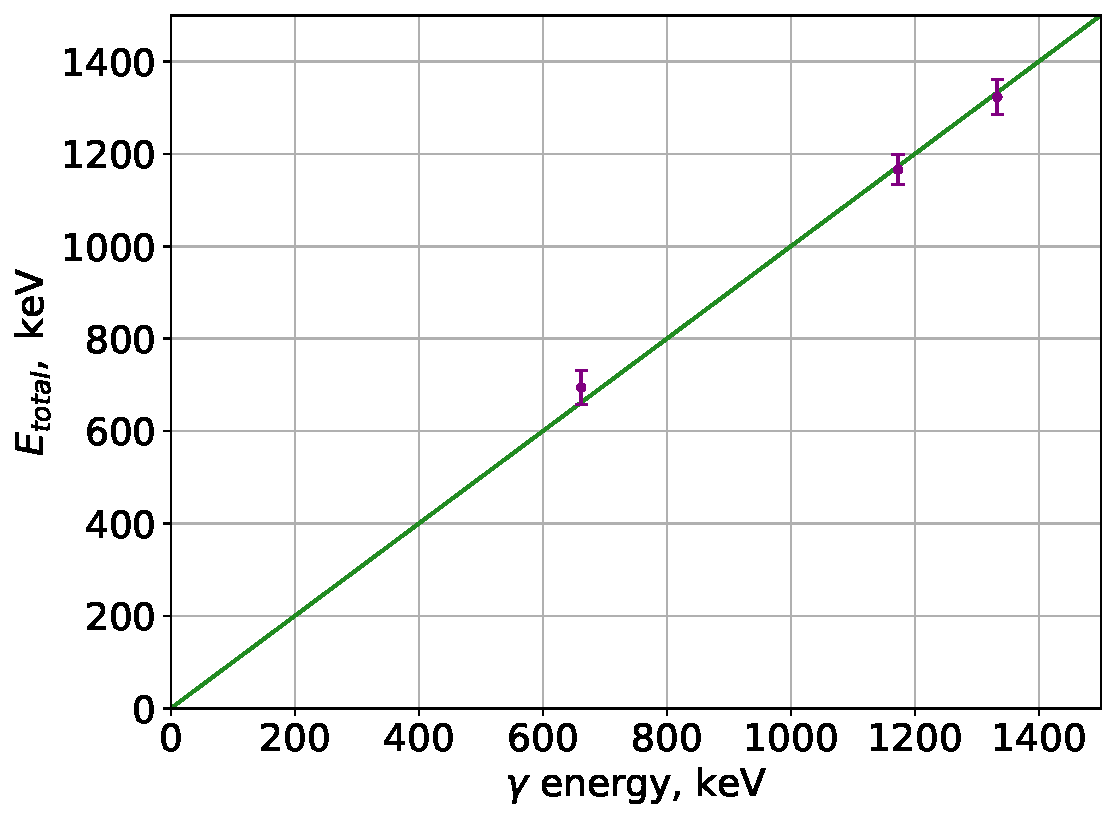
\includegraphics[width=1.0\linewidth]{images/calibr2022.pdf} \\}
  \end{minipage}
  \hfill
  \begin{minipage}[ht]{0.49\linewidth}  \center{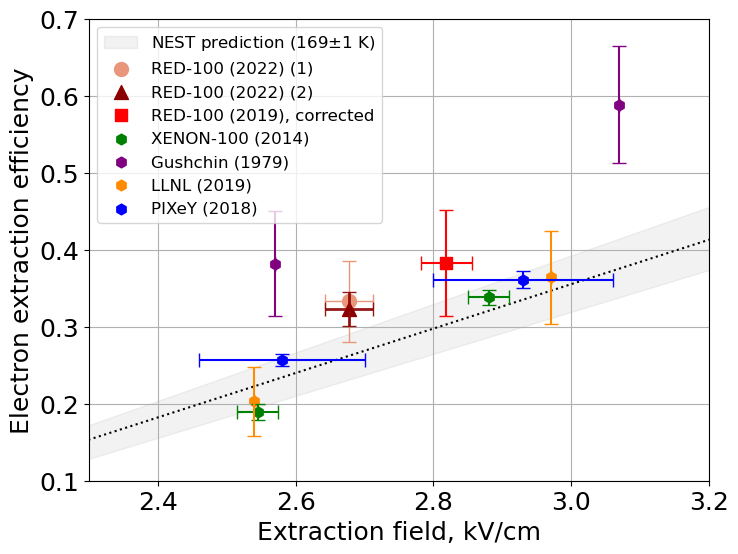
\includegraphics[width=1.0\linewidth]{images/EEEpic.png} \\}
  \end{minipage}
	\caption{\textbf{Left}: $E_{\text{total}}$ versus the $\gamma$-energy \textbf{Right}: Results of EEE evaluation by RED-100 and other experiments~\cite{Gouschin1978,AprileEEE_2014,Edwards_2018, RED100_2019, PhysRevD.99.103024}.}
	\label{img:EEE_SE_rec}
\end{figure}

\begin{table}[hbt]
    \centering
        \caption{Experimental $Q_{\text{el}}$ and $QY$ calculated by NEST}
\begin{tabular}{|c|c|c|}
\hline
    $\gamma$ energy, keV & $Q_{\text{el}}$, e$^-$/keV & NEST $QY$, e$^-$/keV\\
    \hline
    \hspace{0.5em}662 & 13.3$\pm$0.2 & 39.7$\pm$6.0\\
    \hline
    1173 & 13.5$\pm$0.2 & 40.6$\pm$6.2\\
    \hline
    1333 & 13.5$\pm$0.2 & 40.8$\pm$6.4\\
    \hline
\end{tabular}    
\label{tab:IY_table}
\end{table}

In our previous analysis in 2019~\cite{RED100_2019}, we used only the first approach and obtained EEE equal to 54$\pm$8\%. The large discrepancy between previous and current measurements was explained by the introduction of the the SPE area correction coefficient in this work (see section~\ref{subsec:LED}, figure~\ref{img:spe_shape_eff}). Taking into account this coefficient and the updated NEST charge yield (39.7$\pm$6.0~e$^-$/keV instead of 35.6$\pm$3.7~e$^-$/keV), the recalculation of the previous estimate results in 38.5$\pm$6.9\% (red square in figure~\ref{img:EEE_SE_rec}) and lies closer to the NEST prediction.

\section{Conclusion}
\label{sec:concl}
A comprehensive calibration of the RED-100 detector, including several types of measurements, was performed. This paper outlines the data collection, processing, and subsequent analysis methodologies of the calibration data. 
The detector performances based on the \textit{in situ} calibration of single-photon and position-dependent PMT responses have been described.
One of the most significant and useful outcomes of the calibration is the calculation of the LRF shape using an iterative algorithm. 
LRFs can be applied to the position and energy reconstruction of all event types. 
Additionally, knowledge of the LRF shape is essential for detailed signal simulation.

The signals from single ionization electrons have been studied. 
Important parameters such as duration and light yield were obtained. Also, the stability of the detector parameters was monitored, and minor variations were corrected. 
The electron lifetime was measured and is described separately in~\cite{The_RED100_Experiment}. 
Light and charge calibrations were performed using gamma sources. 
Using the combined (S1+S2) energy scale, a good linearity of the response of the RED-100 detector was demonstrated. The EEE value was calculated using two approaches, giving similar results of 33.3$\pm$5.3\% and 32.5$\pm$2.2\% for the extraction electric field of 2.68±0.04 kV/cm. These results are in agreement with those of other experiments and the NEST predictions.


\acknowledgments
The RED-100 project was made possible thanks to administrative support from the State Atomic Energy Corporation Rosatom (ROSATOM) and the Rosenergoatom Joint-Stock Company and financial support from the JSC Science and Innovations (Scientific Division of the ROSATOM) under contract No.313/1679-D dated September 16, 2019 and from the Russian Science Foundation under contract No.22-12-00082 dated May 13, 2022. Authors express their gratitude for the National Research Nuclear University MEPhI (MEPhI Program Priority 2030), the National Research Center “Kurchatov Institute”, the Institute of Nuclear Physics named after G.I. Budker SB RAS, the Tomsk Polytechnic University (Development Program of Tomsk Polytechnic University No. Priority-2030-NIP/EB-004-0000-2022) for support in the development of technology of two-phase emission detectors. This work was funded by the Ministry of Science and Higher Education of the Russian Federation, Project "New Phenomena in Particle Physics and the Early Universe" FSWU-2023-0073. Also, the work was performed with the financial support provided by the Russian Ministry of Science and Higher Education, project “Neutrino detectors for remote monitoring of nuclear power plants and astrophysical installations”, No. FSWU-2022-0018. 

The authors are grateful to the staff of the Kalinin NPP for their continuous organizational and technical support during the RED-100 experiment, as well as the scientists from DANSS, $\nu$GeN, and iDREAM experiments at the Kalinin NPP, for assistance in organizing measurements.


% Bibliography

%% [A] Recommended: using JHEP.bst file
\bibliographystyle{JHEP}
\bibliography{biblio.bib}

%% or
%% [B] Manual formatting (see below)
%% (i) We suggest to always provide author, title and journal data or doi:
%% in short all the informations that clearly identify a document.
%% (ii) please avoid comments such as "For a review'', "For some examples",
%% "and references therein" or move them in the text. In general, please leave only references in the bibliography and move all
%% accessory text in footnotes.
%% (iii) Also, please have only one work for each \bibitem.

%%\begin{thebibliography}{99}

%%\bibitem{a}
%%Author,
%%\emph{Title},
%%\emph{J. Abbrev.} {\bf vol} (year) pg.

%%\bibitem{b}
%%Author,
%%\emph{Title},
%%arxiv:1234.5678.

%%\bibitem{c}
%%Author,
%%\emph{Title},
%%Publisher (year).

%%\end{thebibliography}
\end{document}
